\documentclass[english,gradu]{tktltiki2018}
\usepackage{epsfig}
%\usepackage[pdftex]{graphicx}
\usepackage{url}
\usepackage{lmodern}
\usepackage{microtype}
\usepackage{amsfonts,amsmath,amssymb,amsthm,booktabs,color,enumitem,graphicx,mathabx}
\usepackage{subcaption,xspace}
\usepackage{cleveref}
\usepackage{algpseudocode}
\begin{document}
\onehalfspacing

\newtheorem{theo}{Theorem}
\newtheorem{lem}{Lemma}[section]
\newtheorem{cor}[lem]{Corollary}

\theoremstyle{definition}
%\newtheorem{def}[theo]{Definition}
\newtheorem{prob}{Problem}
\newtheorem{alg}{Algorithm}[section]
\newtheorem{ex}{Example}

\theoremstyle{remark}
\newtheorem*{note}{Remark}

\newcommand\range[2]{\ensuremath{\left [ #1 , #2 \right )}\xspace}
\newcommand\orange[2]{\ensuremath{\left ( #1 , #2 \right )}\xspace}
\newcommand\crange[2]{\ensuremath{\left [ #1 , #2 \right ]}\xspace}
\newcommand\set[1]{\ensuremath{\left\{#1\right\}}\xspace}
\newcommand\size[1]{\ensuremath{\left |#1\right |}\xspace}
\newcommand\ceil[1]{\ensuremath{\left\lceil #1\right\rceil}\xspace}
\newcommand\reals{\ensuremath{\mathbb{R}}\xspace}

\newcommand\spt{\ensuremath{\textbf{s}}\xspace}
\newcommand\ept{\ensuremath{\textbf{t}}\xspace}
\newcommand\fspace{\ensuremath{\mathcal{A}}\xspace}
\newcommand\dirs{\ensuremath{\mathcal{C}}\xspace}

\newcommand\epts{\ensuremath{P}\xspace}
\newcommand\segsize{\ensuremath{n}\xspace}
\newcommand\inter[1]{\ensuremath{\textsc{intr}(#1)}\xspace}
\newcommand\leftc[1]{\ensuremath{\textsc{left}(#1)}\xspace}
\newcommand\rightc[1]{\ensuremath{\textsc{right}(#1)}\xspace}
\newcommand\leftu[2]{\ensuremath{\textsc{fst}_{#2}(#1)}\xspace}
\newcommand\rightu[2]{\ensuremath{\textsc{snd}_{#2}(#1)}\xspace}
\newcommand\reach[1]{\ensuremath{\textsc{reach}(#1)}\xspace}
\newcommand\canon[1]{\ensuremath{\textsc{c}(#1)}\xspace}
%\newcommand\canonp[1]{\ensuremath{\dot{\textsc{c}}(#1)}\xspace}
%\newcommand\canont[2]{\ensuremath{\textsc{c}(#1,#2)}\xspace}
\newcommand\canoni[2]{\ensuremath{\textsc{c}_{#2}(#1)}\xspace}
\newcommand\canonpar[1]{\ensuremath{\textsc{a}_{\textsc{c}}(#1)}\xspace}
\newcommand\canonpari[2]{\ensuremath{\textsc{a}_{\textsc{c},#2}(#1)}\xspace}
\newcommand\epar[1]{\ensuremath{\textsc{p}(#1)}\xspace}
\newcommand\findol{\ensuremath{\textsc{FindOverlapping}}\xspace}
\newcommand\visitp{\ensuremath{\textsc{VisitAncestor}}\xspace}
\newcommand\visitc{\ensuremath{\textsc{VisitCanonical}}\xspace}
\newcommand\adddt{\ensuremath{\textsc{InsertToTree}}\xspace}
\newcommand\checkdt{\ensuremath{\textsc{QueryTree}}\xspace}
\newcommand\cleariv{\ensuremath{\textsc{ClearInterval}}\xspace}
\newcommand\maskof[1]{\ensuremath{\textsc{NodeMask}(#1)}\xspace}
\newcommand\cleardt{\ensuremath{\textsc{ClearFromTree}}\xspace}
\newcommand\clearst{\ensuremath{\textsc{ClearSubtree}}\xspace}
\newcommand\pdst{\ensuremath{\textsc{PushDownSubtree}}\xspace}
\newcommand\recomp{\ensuremath{\textsc{RecomputeSubtreeData}}\xspace}

\newcommand\nodecs[1]{\ensuremath{\textsc{ic}(#1)}\xspace}
\newcommand\nodeps[1]{\ensuremath{\textsc{ip}(#1)}\xspace}
\newcommand\subtree[1]{\ensuremath{\texttt{subtree}(#1)}\xspace}
\newcommand\subtreep[1]{\ensuremath{\texttt{subtreeP}(#1)}\xspace}
\newcommand\hasrect[1]{\ensuremath{\texttt{hasrect}(#1)}\xspace}
\newcommand\hasbits[2]{\ensuremath{\texttt{hasbits}(#1)[#2]}\xspace}
\newcommand\hasbita[1]{\ensuremath{\texttt{hasbits}(#1)}\xspace}

\newcommand\rect[1]{\ensuremath{\textsc{rect}(#1)}\xspace}

\newcommand\pop[1]{\ensuremath{\textsc{pop}(#1)}\xspace}

\newcommand\y[1]{\ensuremath{{#1}_y}\xspace}
\newcommand\x[1]{\ensuremath{{#1}_x}\xspace}
\newcommand\xrange[1]{\ensuremath{x(#1)}\xspace}
\newcommand\yrange[1]{\ensuremath{y(#1)}\xspace}
\newcommand\zrange[1]{\ensuremath{z(#1)}\xspace}
\newcommand\xranget[2]{\ensuremath{x(#1)_{#2}}\xspace}
\newcommand\yranget[2]{\ensuremath{y(#1)_{#2}}\xspace}
\newcommand\zranget[2]{\ensuremath{z(#1)_{#2}}\xspace}
\newcommand\dranget[2]{\ensuremath{D(#1)_{#2}}\xspace}
\newcommand\nbs[1]{\ensuremath{\textsc{nbs}{(#1)}}\xspace}
\newcommand\nbsd[2]{\ensuremath{\textsc{nbs}_{#2}{(#1)}}\xspace}
\newcommand\obsd[2]{\ensuremath{\textsc{obs}_{#2}{(#1)}}\xspace}

\newcommand\decomp[1]{\ensuremath{\textsc{dec}_{#1}}\xspace}
%\newcommand\decompc[1]{\ensuremath{\textsc{dec}({#1})}\xspace}
\newcommand\sweep[2]{\ensuremath{\textsc{sweep}_{#2}{(#1)}}\xspace}
\newcommand\stepof[1]{\ensuremath{\textsc{step}{(#1)}}\xspace}
\newcommand\proj[2]{\ensuremath{\text{proj}_{#1}(#2)}\xspace}

\newcommand\rotr[1]{\ensuremath{\top #1}\xspace}
\newcommand\vecof[1]{\ensuremath{\left [#1\right ]}\xspace}
\newcommand\sline[1]{\ensuremath{S_{#1}}\xspace}
\newcommand\intert[2]{\ensuremath{\textsc{interval}_{#1}(#2)}\xspace}
\newcommand\point[1]{\ensuremath{\left ({#1}\right )}\xspace}

\newcommand\cellE{\ensuremath{\mathsf{CellEvent}}\xspace}
\newcommand\cellEs{\ensuremath{\mathsf{CellEvent}}s\xspace}
\newcommand\obsE{\ensuremath{\mathsf{ObstacleEvent}}\xspace}
\newcommand\obsEs{\ensuremath{\mathsf{ObstacleEvent}}s\xspace}
\newcommand\addE{\ensuremath{\mathsf{AddRangeEvent}}\xspace}
\newcommand\addEs{\ensuremath{\mathsf{AddRangeEvent}}s\xspace}
\newcommand\cellof[1]{\ensuremath{\text{cell}(#1)}\xspace}
\newcommand\rectof[1]{\ensuremath{\text{rect}(#1)}\xspace}
\newcommand\hrectof[1]{\ensuremath{\text{hyperrect}(#1)}\xspace}


\title{Rectilinear minimum link paths in two and higher dimensions}
\author{Mikko Sysikaski}
\date{\today}
\level{Master's thesis}

\maketitle

\numberofpagesinformation{\numberofpages\ pages + \numberofappendixpages\ appendices}

\classification{\protect{\ \\
%\  General and reference $\rightarrow$ Document types  $\rightarrow$ Surveys and overviews\  \\
%\  Applied computing  $\rightarrow$ Document management and text processing  $\rightarrow$ Document management $\rightarrow$ Text editing\\
F.2.2 [Nonnumerical Algorithms and Problems]}}

\keywords{algorithms, computational geometry, route planning}

\supervisors{Antti Laaksonen and Jyrki Kivinen}

\additionalinformation{Thesis for the Algorithms, Data Analytics and Machine Learning subprogramme}

\begin{abstract}
The thesis subject are algorithms for the minimum link path problem.
The minimum link path problem is a well known geometric path finding problem.
The goal is to find a path that does the minimum number of turns amidst obstacles in a plane.
We focus on the rectilinear variant of the problem, where the path and the obstacles are restricted to the directions of the coordinate axes.

We study the rectilinear minimum link path problem in plane and in three-dimensional space, as well as in higher dimensional domains.
We develop new algorithms for the 3D and the high-dimensional case that achieve better asymptotic running times than the previous known methods.
We present an algorithm for the 3D rectilinear path problem with running time $O(n^2\log^2 n)$ and space complexity $O(n^2)$ in a domain with $n$ obstacle vertices.
We show that the solution can be generalized to higher dimensions, leading to an algorithm for the $D$-dimensional minimum link path problem with $O(n^{D-1}\log^{D-1} n)$ running time and $O(n^{D-1})$ space complexity.
\end{abstract}

\mytableofcontents


\section{Introduction}

Various kinds of path finding problems are an extremely common topic in algorithmics~\cite{survey}.
The regular shortest path problem asks for the shortest path between two nodes in a graph.
The geometric version of the problem asks for the shortest path in a continuous space, such as a plane with polygonal obstacles.
The typical goal is to minimize the Euclidean length of the path, but for some applications other distance metrics are also relevant.
For example a robot might move forward quickly but turn very slowly, so a long simple route is sometimes preferable to a shorter but more complex route.

The topic of this thesis is finding geometric path that minimize the amount of points where the path takes a turn.
Consider a path consisting of a finite number of straight line segments, also called \emph{links}.
The \emph{link distance} of the path is the number of segments.
A \emph{minimum link path} between two points is a path that minimizes the link distance.
Figure~\ref{fig:paths} shows an example of two kinds of minimum link paths as well as the regular shortest path.

\begin{figure}\centering
	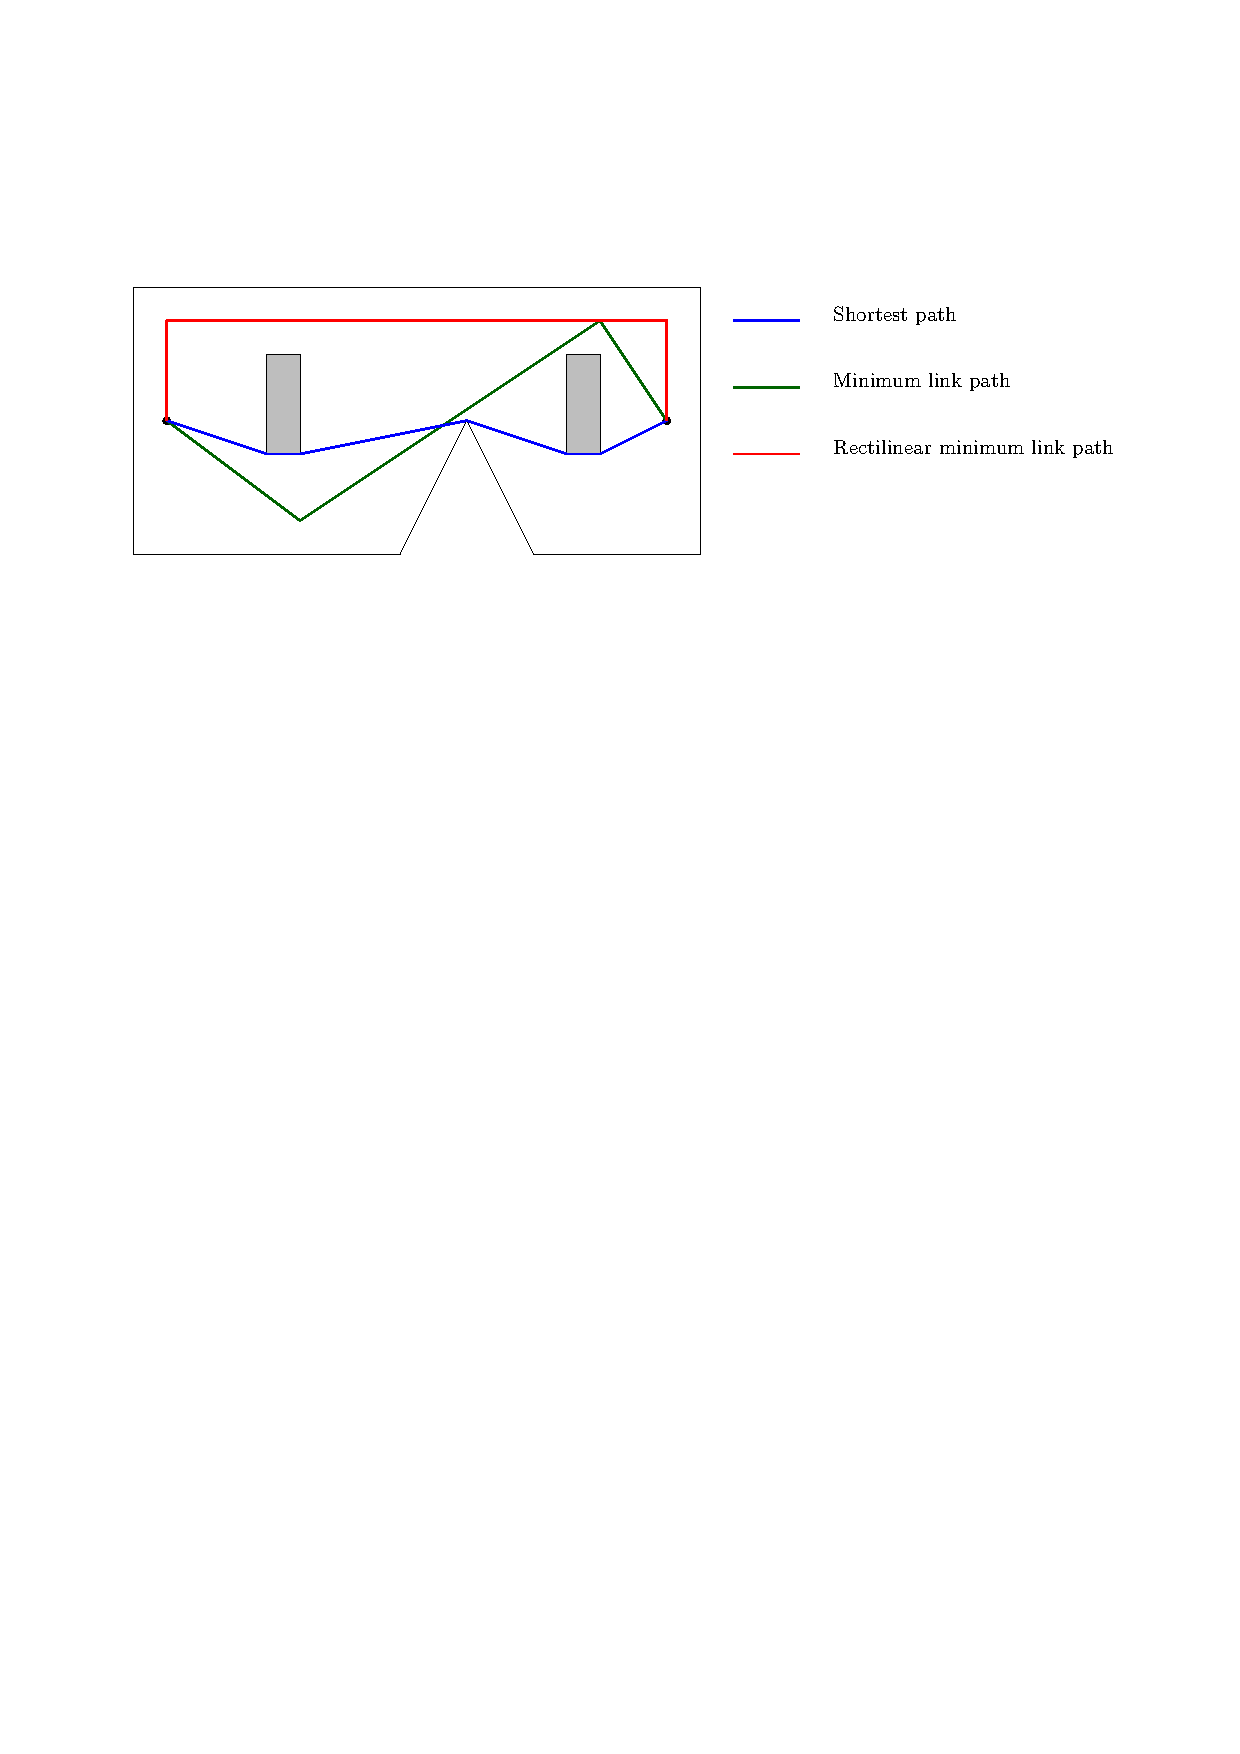
\includegraphics[width=\textwidth]{fig/paths}
	\caption{There are many variants of the geometric path finding problem, producing different kinds of paths.}\label{fig:paths}
\end{figure}

Finding minimum link paths is a well studied algorithmic problem\cite{restricted,wagner,dasnar,de1991,de1992,fitch,handbook}.
The basic idea employed by most known algorithms is a simple extension of the breadth-first search:
First find all the points that have link distance~1 from the starting point, then points with link distance~2, and similarly iterate until the desired endpoint is encountered.
As the search happens in continuous space, the tricky part of the algorithms is defining the appropriate data structures to store and update the discovered area.

In this thesis we focus on the \emph{rectilinear} variant of the problem.
In the rectilinear minimum link path problem the obstacles as well as the links of the paths are restricted to coordinate axes' directions.
We study both the planar case as well as 3D version of the rectilinear minimum link path problem.
We present a new algorithm for the 3D case with $O(n^2\log^2n)$ running time, which is a significant improvement over the earlier best known result $O(n^{2.5}\log n)$~\cite{restricted}.
Finally, we extend the solution to work in any $D$-dimensional rectilinear domain, resulting in an algorithm with time complexity $O(n^{D-1}\log^{D-1}n)$.

\subsection{Background and new results}

Computing rectilinear minimum link paths is an old and well studied problem.
The problem was presented in 1968 by Mikami and Tabuchi~\cite{mikami}, who also gave an algorithm with $O(n^2)$ running time.
Sato, Sakanaka and Ohtsuki~\cite{sato} presented an algorithm with $O(n\log n)$ time and $O(n)$ space.
A similar result was achieved independently by Das and Narasimhan~\cite{dasnar}.
These results are asymptotically optimal, as the problem can be shown to be as hard as sorting~\cite{dasnar} and thus having lower bound $O(n\log n)$.

Several algorithms have also been developed for the higher dimensional rectilinear minimum link path problem.
De Berg et al.~\cite{de1992} gave an $O(n^D\log n)$ algorithm for the $D$-dimensional minimum link path problem.
For the 3D case, an $O(n^3)$ algorithm was developed by Mikami and Tabuchi~\cite{mikami}.
Fitch, Butler and Rus~\cite{fitch} gave an algorithm which improves the performance in many cases, but still has $O(n^3)$ worst case running time.
This was further improved by Wagner, Drysdale and Stein~\cite{wagner}, who gave an algorithm with worst case time complexity $O(n^{2.5}\log n)$.

In this thesis we focus on new results to the rectilinear minimum link path problem, which are original research of the author.
The following results have been published in peer-reviewed journals and conferences.
\begin{itemize}
\item A simplified $O(n\log n)$ algorithm for the 2-dimensional case~\cite{revisited}.
The article was written with the co-authors Valentin Polishchuk and Joseph S. B. Mitchell.
The main algorithmic ideas of the algorithm were invented by the author, though many details of it were worked out with Polishchuk.
The contribution of Mitchell was mainly for other results not discussed in this thesis, such as the approximation algorithm for the non-rectilinear minimum link path problem.
\item A new algorithm for the 3D minimum link path problem, improving the running time from the previous best result of $O(n^{2.5}\log n)$ to $O(n^2\log^2 n)$~\cite{restricted}.
The publication was written with the co-author Valentin Polishchuk.
The main algorithmic ideas were invented by the author, but many details and proofs of the running time were worked out together with Polishchuk.
\end{itemize}

The following items are new original contributions in this thesis.

\begin{itemize}
\item An algorithm for the minimum link path problem in higher dimensions.
	We show that the rectilinear minimum link path problem in $D$ dimensions can be solved in $O(n^{D-1}\log^{D-1} n)$ time by a generalization of the 3D algorithm.
\item Detailed description of the algorithm for 3D minimum link path computation and the data structures used in the algorithm.
\item Extension of the space decomposition used in the 3D algorithm to higher dimensions.
\item Simplification of the 3D minimum link algorithm by using the unified segment tree by Wagner~\cite{unified}.
\item Extending the unified segment tree to higher than 2 dimensions and showing how to clearing a hyperrectangle in the tree.
	The original paper by Wagner~\cite{unified} mentions the possibility of extending the structure to higher dimensions, but does not provide any details.
\end{itemize}

\subsection{Overview of the algorithms}\label{sec:overview}

Majority of the known algorithms for the minimum link path problem use the same basic idea~\cite[Sections 26.4, 27.3]{handbook}:
The tasks is to find a minimum link path from point \spt to point \ept within free space~\fspace.
The free space is the area not blocked by any obstacles.
Let \reach{k} be the set of points reachable by at most $k$ links from \spt.
We start by defining $\reach{0}=\set{\spt}$, and iteratively compute \reach{k+1} from \reach{k}.
The iteration continues until we find $k$ such that $\ept\in\reach{k}$.
This iteration is often called \emph{staged illumination}, because the computation of \reach{k+1} can be illustrated as placing light sources on the boundaries of \reach{k}.
Figure~\ref{fig:staged} shows an example of the staged illumination process.

\begin{figure}\centering
	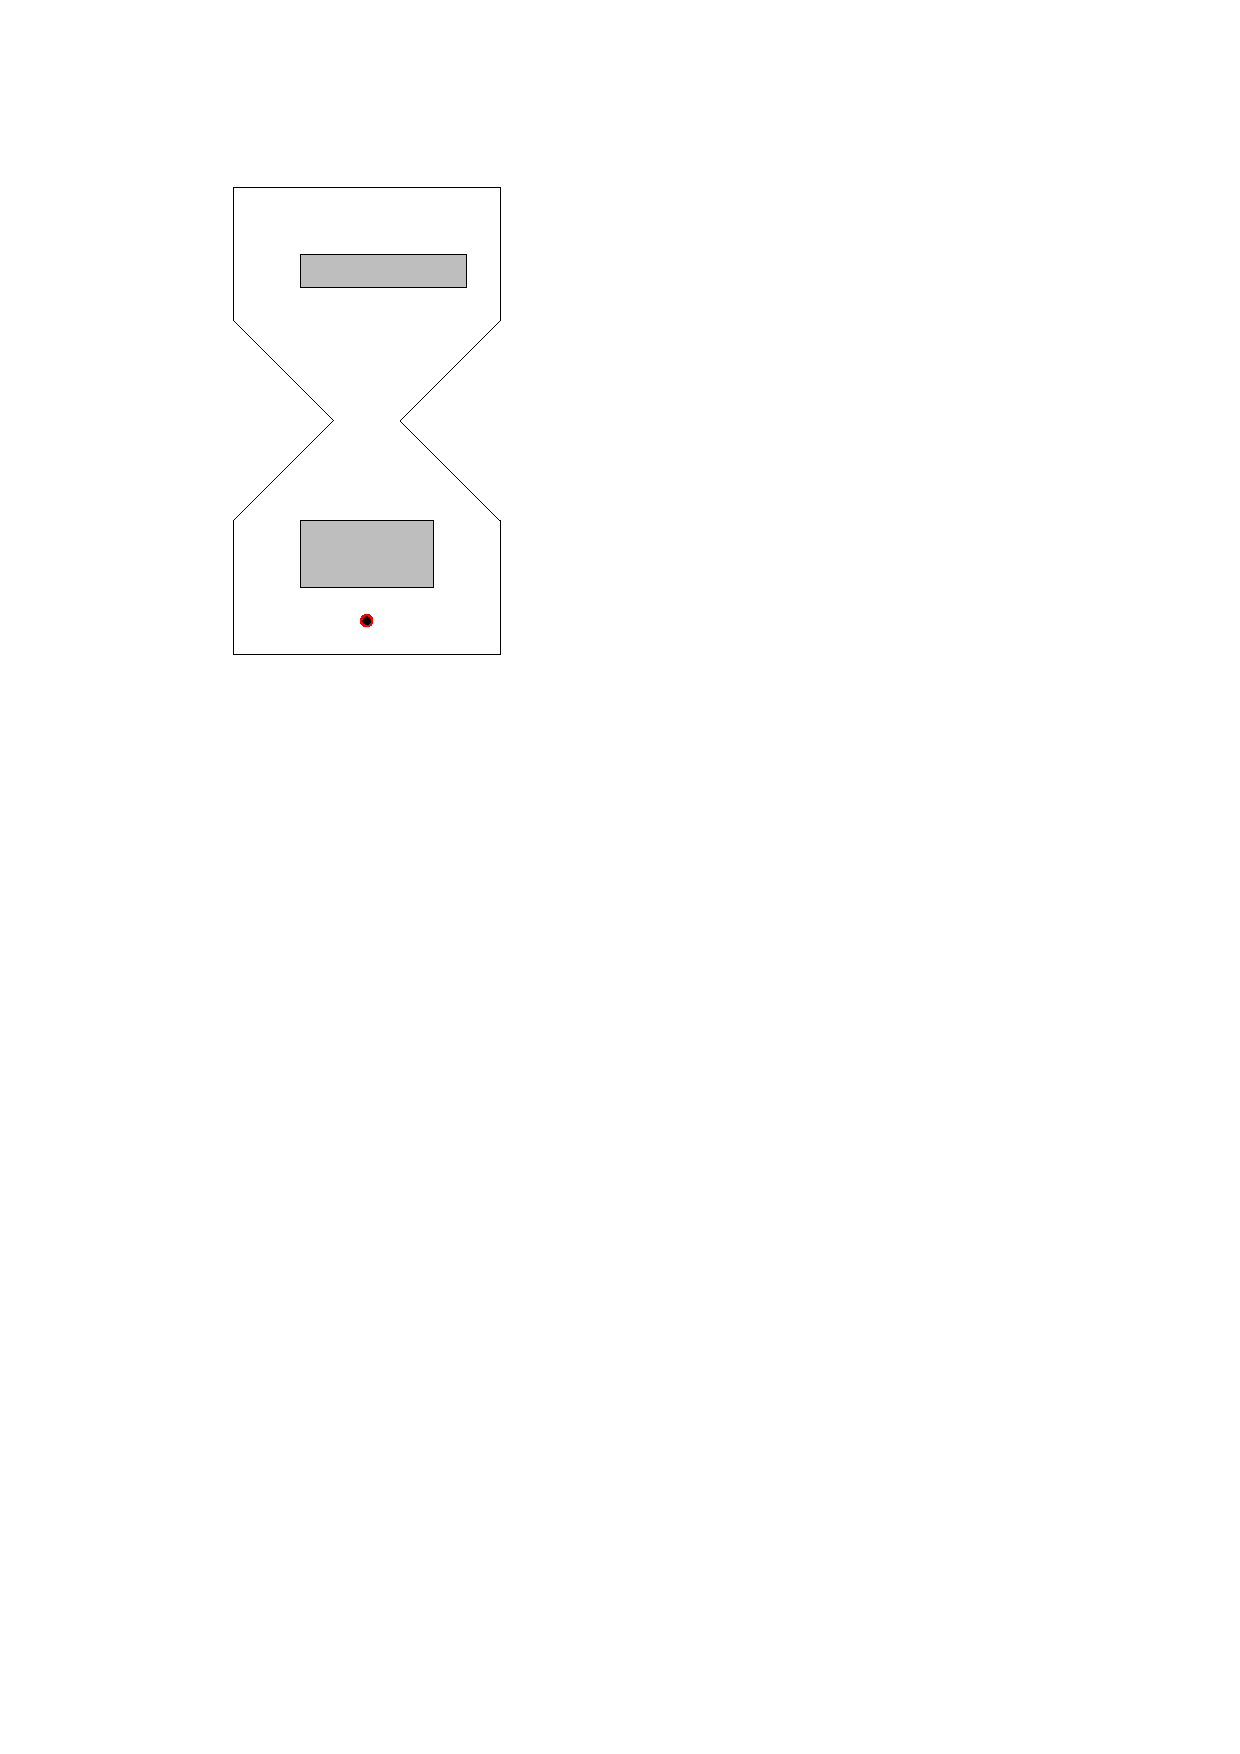
\includegraphics[scale=0.5,page=1]{fig/staged}
	\hfil
	\includegraphics[scale=0.5,page=2]{fig/staged}
	\hfil
	\includegraphics[scale=0.5,page=3]{fig/staged}
	\hfil
	\includegraphics[scale=0.5,page=4]{fig/staged}
	\caption{Four steps of staged illumination from a single starting point. The new areas are illuminated through the red boundaries on each step.}\label{fig:staged}
\end{figure}

The illumination process closely resembles the breadth-first search, though with a key difference that the search is done in a continuous space rather than in a graph.
A nontrivial part of the minimum link path algorithms is maintaining the illuminated area in a data structure that allows efficient computation of \reach{k+1} from \reach{k}.

Representing the illuminated area can be simplified by first splitting the free space into rectangles.
This is analogous to how many problems in computational geometry are solved by first triangulating the input~\cite{handbook}.
In Section~\ref{sec:decomposition} we present an algorithms for construction a decompositions suitable for the minimum link path computation.

Because the possible directions of the links of the path are limited, we can use \emph{sweep line algorithms} to efficiently compute \reach{k+1} from \reach{k}.
Sweep line algorithms are a generic technique used for a wide range of computational geometry problems~\cite[Section 33.2]{clrs}.
The idea is to image a line that crosses over the domain and stops at some discrete \emph{events}.
As the sweep line progresses, we gradually update the solution to take into account the parts of the domain encountered in the events.
The sweep line method allows us to transform the 2-dimensional illumination problem into a series of easier 1-dimensional problems on the sweep line.

During the sweeps we need to maintain the relationship between the sweep line and the obstacles as well as the region \reach{k}.
We want to maintain the intersection of the sweep line with the illuminated area, which requires efficient handling of number intervals.
\emph{Segment tree} is a generic data structure for working with intervals.
It is flexible enough to allow implementing all the operations required by the staged illumination.
Segment trees are described in Section~\ref{sec:segtree}.

We combine the aforementioned concepts into a simple algorithm for finding minimum link paths in Section~\ref{sec:minlink2d}.
The ideas of the two-dimensional solution can also be generalized to work in higher dimensions.
Many details need to be taken care of, but the basic ideas are relatively straightforward to transfer to more than two dimensions.
The space is decomposed into cuboids instead of rectangles, and the sweep line is replaced by a sweep plane.
The segment tree can also be generalized into a higher dimensional structure.
These elements are combined into an algorithm for finding minimum link paths in three and higher dimensional domains in Section~\ref{sec:minlink3d}.



\section{Space decomposition}\label{sec:decomposition}

The first step of many minimum link path algorithms is decomposing the free space into simple primitives~\cite{imai86,dasnar,revisited}.
The decomposition has two purposes during the staged illumination:
to track the illuminated area and to guide the sweep line algorithms that illuminate new areas.

%The domain of the minimum link path problem is a polygon with smaller polygons as obstacles.
%The input is given as a list of polygons, and each polygon is described by a list of vertices.
%This form is inconvenient for path planning algorithms, as many simple operations, such as checking whether we can move from a given point to a given direction, require scanning through all the polygons.

In the rectilinear minimum link path problem the obstacle edges are oriented according to the coordinate axis.
This allows us to decompose the free space into axis-aligned rectangles, which is a convenient form for rectilinear path computation.
For each cell of the decomposition we also construct links to neighboring cells and obstacles.
In other words, the decomposition can be seen as a graph with rectangles as vertices and an edge between each pair of adjacent rectangles.
Let $n$ be the total number of vertices in all the obstacles.
The space can decomposed into $O(n)$ cells such the total number of links between cells is $O(n)$.

A similar structure can also be used for computing minimum link paths in 3-dimensional domains.
In the 3D rectilinear case each obstacle face is an axis-aligned rectangle in 3D space.
The free space of a 3D domain can be decomposed into a graph with $O(n^2)$ cuboid as vertices and $O(n^2)$ edges.
This decomposition algorithm can also be extended to higher dimensions: a $D$-dimensional domain can be split into $O(n^{D-1})$ hyperrectangles with $O(n^{D-1}$ links between them.

\subsection{Planar decomposition}\label{sec:decomp2d}

A rectilinear domain can be decomposed into rectangles by extending each horizontal obstacle edge in both directions until the sides hit a vertical obstacle edge~\cite{imai86}.
This defines the \emph{horizontal decomposition} of the domain, denoted \decomp{x}.
The vertical decomposition \decomp{y} is defined correspondingly by extending all the vertical edges until they hit a horizontal obstacle.
Figure~\ref{fig:decomp} shows an example of the two two decompositions.
We focus on \decomp{x} below, as \decomp{y} has all the same properties with coordinate axes swapped.

\begin{figure}\centering
	
\includegraphics[scale=0.6,page=2]{fig/decomp}
	\hfil
	
\includegraphics[scale=0.6,page=3]{fig/decomp}
	\caption{Horizontal and vertical decomposition of the same domain. Each cell touches at least one obstacle corner and each obstacle corner touches at most two cells, so both decompositions have size $O(n)$.}\label{fig:decomp}
\end{figure}

It is easy to see that each cell of \decomp{x} touches at least one obstacle vertex.
Since each vertex can be touched by at most two rectangles, the size of the decomposition is $O(n)$.
Each pair of touching rectangles also shares a common obstacle corner, so the number of links is also $O(n)$.

\decomp{x} can be constructed by a line sweep algorithm~\cite{dasnar}.
We sweep over the domain by a horizontal line moving from $y$ coordinate $-\infty$ (down) to $\infty$ (up).
During the sweep we maintain the intersection of the free space \fspace and the sweep line.
The intersection consists of non-overlapping intervals, which we store in a binary search tree.
Each element added to the binary tree is a rectangle $a$ defined by intervals \xrange{a} and \yrange{a}.
We refer to lower and upper bound of each range $r$ by $r_{start}$ and $r_{end}$.
\yranget{a}{end} is initially undefined when a rectangle $a$ is added to the tree, because we don't know how tall the rectangle will be until $a$ is removed from the tree.

The sweep stops at each horizontal obstacle edge.
When moving from down to up, each edge starts either starts or ends an obstacle.
If the edge starts an obstacle, the $x$-range of the edge is fully contained in one of the intervals in the search tree.
If the edge ends an obstacle, the $x$-range does not intersect any intervals in the tree, but the left and right endpoints may touch some intervals.
In both cases the rectangles touching the encountered edge are removed from the search tree, and $O(1)$ new rectangles are inserted to maintain the sweep line state.
A more exact description of the algorithm follows below.

\begin{alg}\label{alg:split2d}
Decompose the free space defined by a set $E$ of obstacle edges into \decomp{x}.
\begin{algorithmic}
\State $T\gets \text{Empty binary search tree}$.
\State Sort $E$ by the $y$ coordinates of the edges.
\ForAll{$e\in E$}
	\If{$e$ starts an obstacle}
		\Comment Exactly one $x$-interval in $T$ intersects \xrange{e}.
		\State $v\gets\text{Lookup $T$ for interval touching \xrange{e}}$.
		\State Remove $v$ from $T$.
		\State $\yranget{v}{end}\gets\y{e}$.
		\ForAll{$u\gets \xrange{v}\setminus \xrange{e}$}
			\Comment Loop over remaining parts of the entry removed from $T$.
			\State $a\gets$ New rectangle with $x$-range $u$ and starting $y$-coordinate $\y{e}$.
			\State Insert $a$ into $T$.
		\EndFor
	\Else\Comment $e$ starts free space.
		\State $a\gets$ New rectangle.
		\State $a\gets$ New rectangle with $x$-range $\xrange{e}$ and starting $y$-coordinate $\y{e}$.
		\ForAll{$v\in$ lookup $T$ for intervals touching \xrange{e}}
			\State Remove $v$ from $T$.
			\State $\yranget{v}{end}\gets\y{e}$.
			\State $\xrange{a}\gets\xrange{a}\cup\xrange{v}$.
		\EndFor
		\State Insert $a$ into $T$.
	\EndIf
\EndFor
\end{algorithmic}
\end{alg}

In addition to the cells, we also want to compute the links between all adjacent pairs.
It is straightforward to extend Algorithm~\ref{alg:split2d} to compute the links by inserting links between the cells that are removed and inserted in the binary search tree during each event.
The following lemma gives a bound on the complexity of the algorithm.

\begin{lem}\label{lem:split2dtime}Algorithm~\ref{alg:split2d} works in $O(n\log n)$ time and $O(n)$ space.\end{lem}
\begin{proof}
The algorithm sorts all the horizontal edges in $O(n\log n)$ time and iterates over them in $O(n)$ steps.
On each step we create $O(1)$ new rectangles, and perform $O(1)$ operations to the binary search tree.
The search tree is a balanced binary tree, so each tree operation is carried out in $O(\log n)$ time.
Thus the total complexity of the algorithm is $O(n\log n)$ and we only need $O(n)$ storage for the edge list and the binary search tree as well as for storing the output.
\end{proof}

\subsection{3D cuboid decomposition}\label{sec:split3d}

As a 2D domain can be decomposed into rectangles, a 3D rectilinear domain can be decomposed into cuboids~\cite{wagner,restricted}.
Decomposition into cuboids is used in the algorithm for 3D minimum link paths in Section~\ref{sec:minlink3d}.
The running time of the path finding algorithm depends on the size of the decomposition, so it is desirable to find as small decomposition as possible.

We present a simple decomposition algorithm that uses the Algorithm~\ref{alg:split2d} as a subroutine~\cite{restricted}.
The algorithm produces a decomposition with $O(n^2)$ cells and $O(n^2)$ links, where $n$ is the number of obstacle rectangles.
Earlier work on minimum link path has used binary space partitioning to reduce the number of cells to $O(n^{1.5})$~\cite{wagner,bsp}.
However the number of links in a binary space partitioning based decomposition can be as high as $O(n^{2.5})$, so we opt for a higher number of cells to reduce the number of links.

The decomposition is created by a sweep plane algorithm, which sweeps through the domain with a plane perpendicular to $z$-axis.
During the sweep we maintain the intersection of the sweep plane and the domain~\fspace.
The intersection of the domain and a plane is called a \emph{cross section} of the domain.

In each cross section we form a 2D decomposition of the domain with Algorithm~\ref{alg:split2d}, and extend the $xy$-rectangles in $z$-direction so that they fill the whole free space.
Any common rectangles shared by consecutive cross sections are merged into a single larger cuboid.
The merging is done by by maintaining a binary search tree of the cells of the previous decomposition.
Figure~\ref{fig:split3d} shows how the 3D decomposition is created using a series of 2D decompositions.

\begin{figure}\centering
	\begin{subfigure}[t]{0.3\textwidth}\centering
		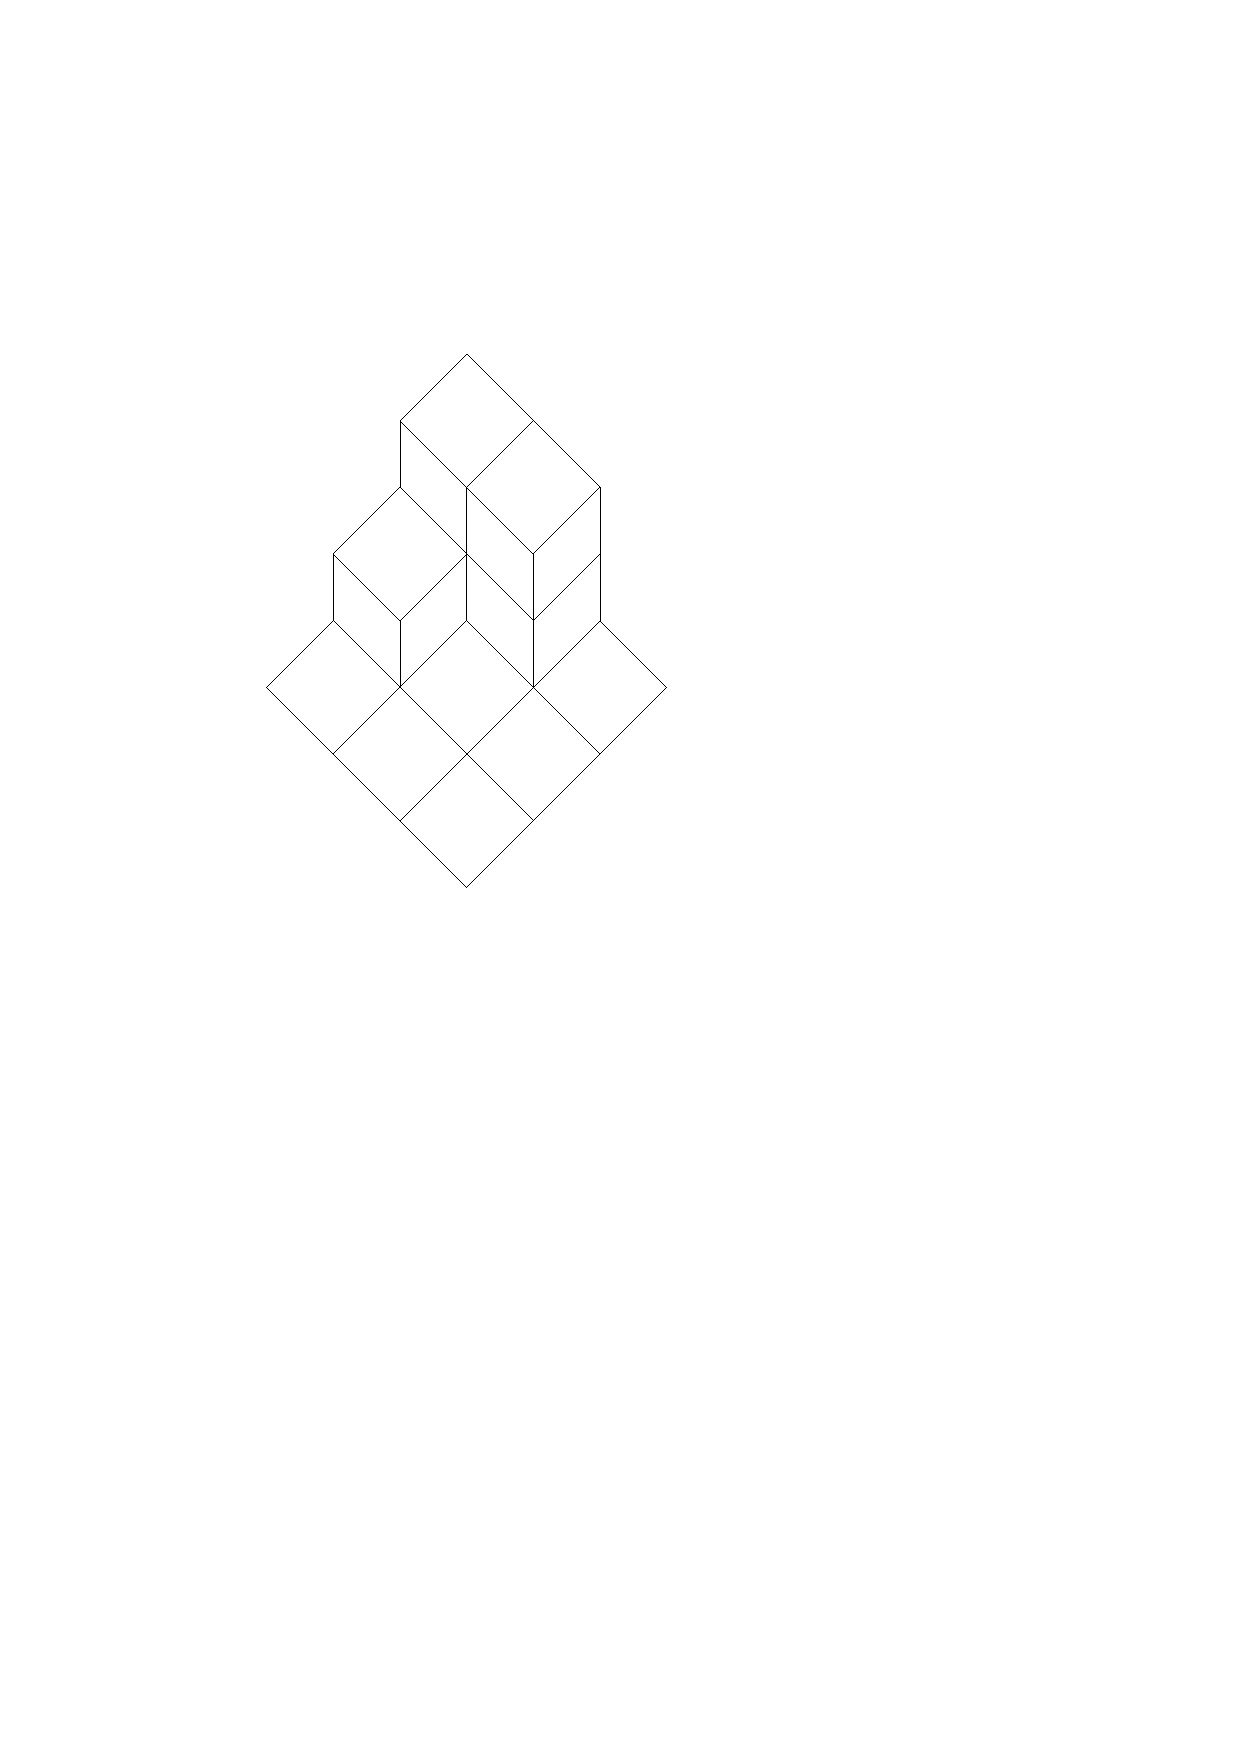
\includegraphics[width=0.5\textwidth,page=1]{fig/split3d}
		\caption{3D domain}
	\end{subfigure}
	\hfil
	\begin{subfigure}[t]{0.3\textwidth}\centering
		\includegraphics[width=0.5\textwidth,page=3]{fig/split3d}
		\caption{Cross section of the lower level}
	\end{subfigure}
	\hfil
	\begin{subfigure}[t]{0.3\textwidth}\centering
		\includegraphics[width=0.5\textwidth,page=4]{fig/split3d}
		\caption{Cross section of the upper level}
	\end{subfigure}
	\caption{3D domain is decomposed into cuboids by taking the horizontal decomposition of each cross section. The highlighted cell is shared between the two cross sections, so the cuboids on the two levels are merged.}\label{fig:split3d}
\end{figure}

The description below only calculates the cells but not the links between them.
We discuss the computation of links below.

\begin{alg}\label{alg:split3d}
Decompose the free space defined by a set $E$ of obstacle faces into cuboids.
\begin{algorithmic}
\State $Z\gets$ All $z$-coordinates of obstacle vertices.
\State Sort $Z$ in increasing order.
\State $R\gets$ Empty list of result cells.
\State $M\gets$ Empty binary search tree mapping 2D rectangles to indices in $R$.
\ForAll{$z\in Z$}
	\State $E_z\gets\set{e \mid e\in E, \zrange{e}\ni z}$.
	\State $T\gets$ 2D decomposition for $E_z$ using Algorithm~\ref{alg:split2d}.
	\ForAll{$m\in M\setminus T$}
		\State $c\gets R[M[m]]$.
		\State $\zranget{c}{end}\gets z$.
		\State Remove $m$ from $M$.
	\EndFor
	\ForAll{$t\in T\setminus M$}
		\State $c\gets$ New cell with $xy$-bounds $t$ and starting $z$-coordinate $z$.
		\State Insert $c$ into $R$.
		\State $M[t]\gets$ index of $c$ in $R$.
	\EndFor
\EndFor
\State Return list $R$.
\end{algorithmic}
\end{alg}

\begin{lem}\label{lem:split3dtime}Algorithm~\ref{alg:split3d} has running time $O(n^2\log n)$.\end{lem}
\begin{proof}
We loop through $O(n)$ unique $z$-coordinates.
For each $z$ we construct a set of obstacles in $O(n)$ time and a 2D decomposition in $O(n\log n)$ time.
The map $M$ is implemented as a binary search tree, so each update and lookup can be performed in $O(\log n)$ time.
For each $z$ we perform $O(n)$ map updates, so the total time complexity is $O(n^2\log n)$.
\end{proof}

Next we show how to compute the links between the cuboids generated by Algorithm~\ref{alg:split3d}.
The following lemma shows how the changes to the cross section affect the number of links.
Figure~\ref{fig:linkproof} illustrates the case where two adjacent cross sections differ by a single obstacle rectangle.

\begin{figure}\centering
	\begin{subfigure}[t]{0.45\textwidth}\centering
		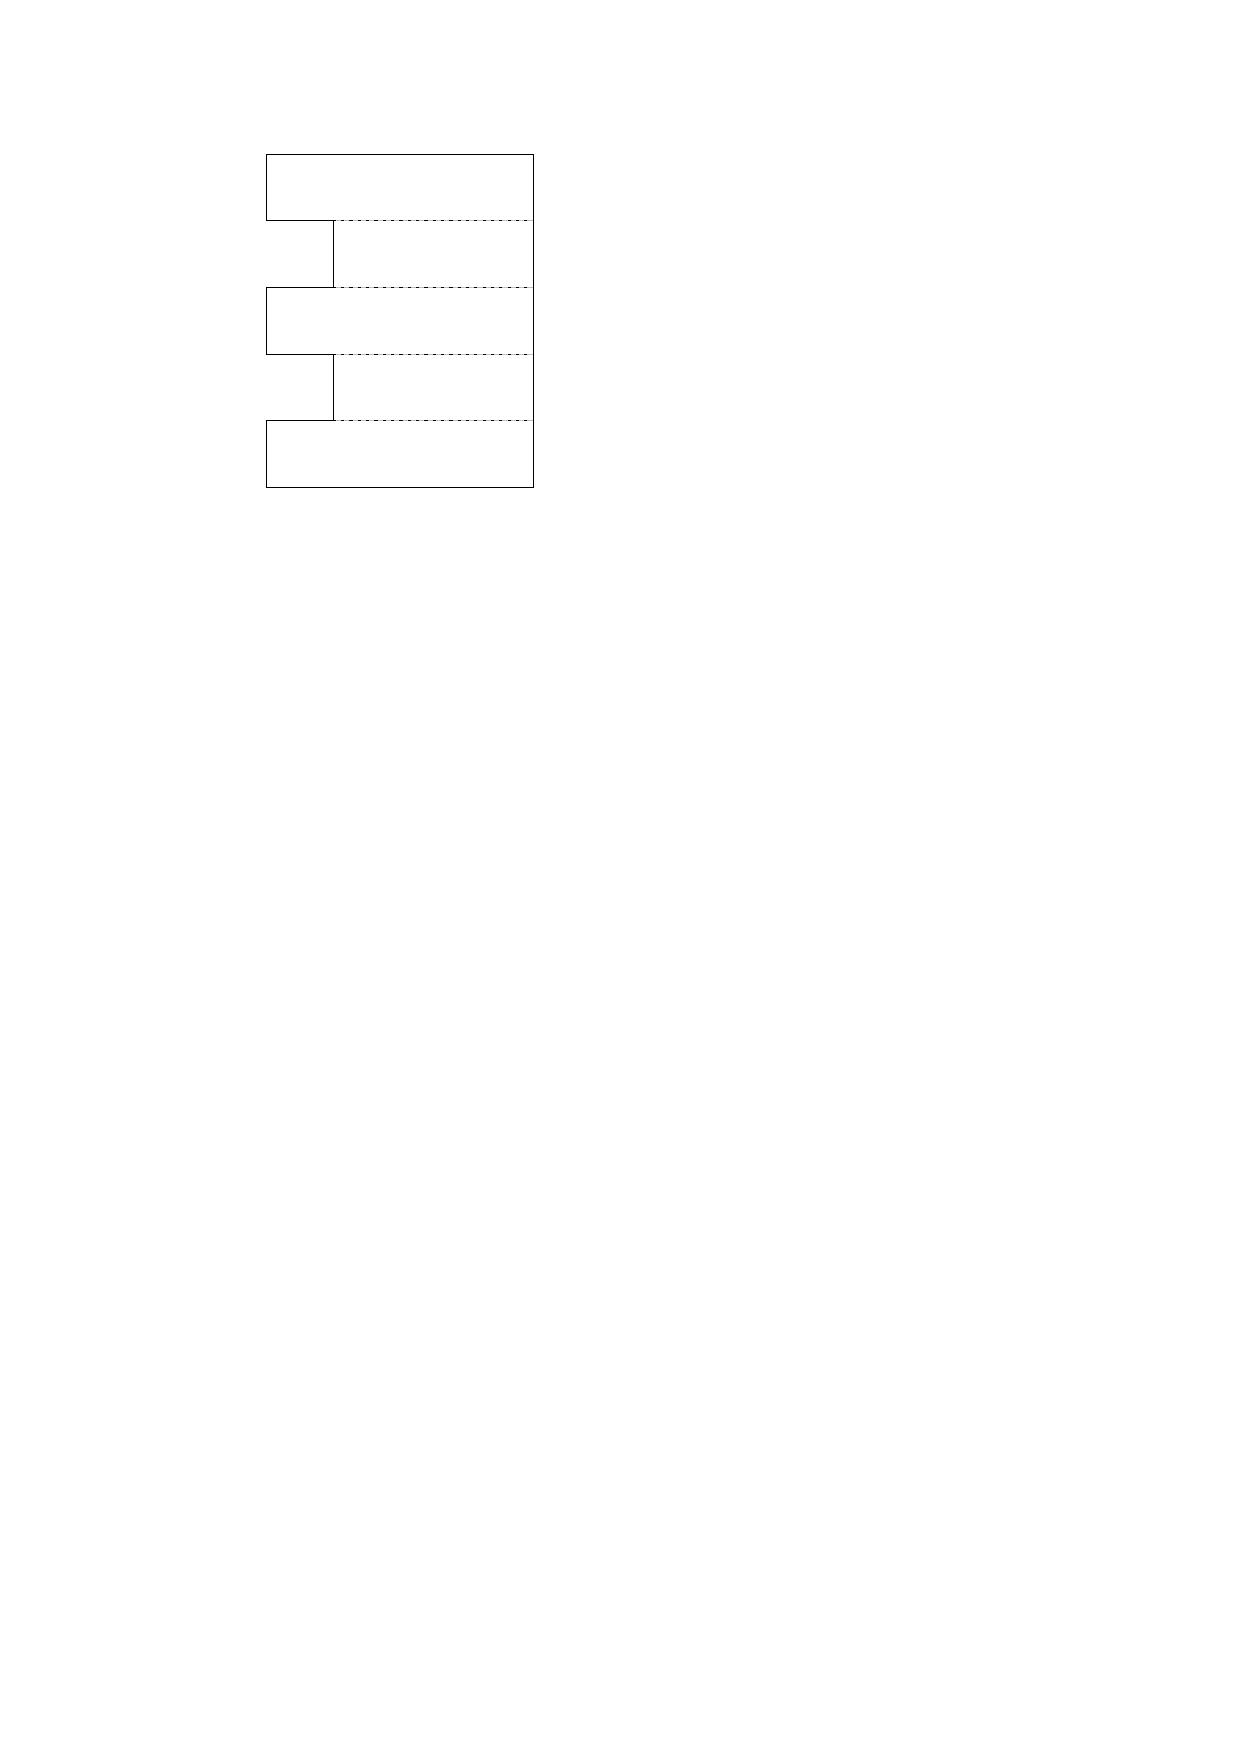
\includegraphics[width=0.5\textwidth,page=1]{fig/linkproof}
		\caption{Original domain}
	\end{subfigure}
	\hfil
	\begin{subfigure}[t]{0.45\textwidth}\centering
		\includegraphics[width=0.5\textwidth,page=2]{fig/linkproof}
		\caption{Domain after adding an obstacle}
	\end{subfigure}
	\caption{Adding or removing a single obstacle can change all $O(n)$ cells of the horizontal decomposition.
	However the intersection of the domain with any horizontal line is changed at only $O(1)$ points.
	Because there are $O(n)$ unique cross sections, the number of overlapping pairs of rectangles in the old and the new domain is $O(n)$.}\label{fig:linkproof}
\end{figure}

\begin{lem}\label{lem:decomp2dch}
Consider two obstacle sets $A$ and $B$ on 2D plane.
Let $n$ be the total number of obstacle edges in $A$ and $B$, and $k$ be the number of edges that are present in exactly one of the sets.
The number of overlapping rectangles in \decomp{x}(A) and \decomp{x}(B) is $O(nk)$.
\end{lem}
\begin{proof}
We divide the intersecting rectangle pairs into two sets:
pairs with identical $x$-range and pairs with different $x$-ranges.
Let $a$ and $b$ be two rectangles with $\xrange{a}=\xrange{b}$.
If $a\cap b\neq\emptyset$, then either $\yranget{a}{start}\in\yrange{b}$ or $\yranget{b}{start}\in\yrange{a}$.
Since the starting $y$-coordinate of any rectangle can be inside only a single rectangle with the same $x$-range, the number of overlapping pairs with equal $x$-range is $O(n)$.

To count the overlapping pairs with different $x$-ranges, consider how the sweep line of Algorithm~\ref{alg:split2d} advances in domains $A$ and $B$.
Recall that the sweep line is a horizontal line moving in $y$-direction.

The intersection of the sweep line and the free space is a sequence of disjoint intervals for both $A$ and $B$.
Since there are $O(k)$ changes to the set of obstacles, the edit distance between the interval sets is $O(k)$ during each point of the sweep.
Thus each $y$ coordinate contributes $O(k)$ pairs to the overlap.
Since the number of $y$ coordinates where the domain changes is $O(n)$, the total number of overlapping pairs is $O(nk)$.
\end{proof}

\begin{lem}\label{lem:split3dcount}The number of pairs of adjacent cells in the decomposition produced by Algorithm~\ref{alg:split3d} is $O(n^2)$.\end{lem}
\begin{proof}
Since the number of links produced by Algorithm~\ref{alg:split2d} is $O(n)$, any cross section has $O(n)$ links in $x$ and $y$ directions.
Thus the total number of $x$ and $y$ links is $O(n^2)$.

Let $k_z$ be the number of obstacles whose $z$-range either starts or ends at $z$.
Since the total number of obstacles is $n$, the sum of $k_z$ values over all $z$-coordinates is $n$.
By Lemma~\ref{lem:decomp2dch} the number of links between two adjacent layers is $O(nk_z)$, so the total number of $z$-links is $\sum_z O(nk_z)=O(n^2)$.
\end{proof}

To generate the links, notice that the links in $x$ and $y$ directions can be simply extracted from the 2D decompositions of each cross section.
What remains is computing the links in $z$ direction.
We compute the links between each pair of adjacent cross sections separately.

Let $A$ and $B$ be the sets of rectangles that are different on the horizontal decompositions of two adjacent cross sections.
Finding the $z$-links in the 3D decomposition is equivalent to finding the set of overlapping pairs between $A$ and $B$.
The pairs are found by running \emph{another} line sweep algorithm after both $A$ and $B$ have been created by Algorithm~\ref{alg:split2d}.

We sweep through the domain again by a horizontal line.
During the sweep we maintain two binary search tree $T_A$ and $T_B$, containing the rectangles of $A$ and $B$ touching the sweep line respectively.
The binary search tree is ordered by the $x$-coordinate of the rectangle.
Note that the rectangles in each of the sets $A$ and $B$ are disjoint, so the $x$-ranges are disjoint as well.

Each time the sweep line arrives into a new rectangle $a\in A$, the tree $T_B$ is queries to find all the rectangles touched by the bottom line of $a$.
Similarly for each new rectangle $b\in B$, we query the tree $T_A$ for rectangles touching the bottom line of $b$.
A more exact description of the algorithm is below.

\begin{alg}\label{alg:overlap2d}
Find all overlapping pairs of two sets of rectangles $A$ and $B$.
\begin{algorithmic}
\State $E\gets$ All bottom and top edges of rectangles in $A$ and $B$.
\State Sort $E$ by $y$-coordinates.
\State $T_A\gets$ Empty binary search tree.
\State $T_B\gets$ Empty binary search tree.
\ForAll{$e\in E$}
	\State $s\in\set{A,B}\gets$ Group to which $e$ belongs to.
	\State $t\in\set{A,B}\gets$ Group to which $e$ does not belong to.
	\If{$e$ starts a rectangle}
		\State Find all elements from $T_t$ with $x$-range intersection the $x$-range of $e$.
		\State Add the rectangle to $T_s$.
	\Else
		\State Remove the rectangle from $T_s$.
	\EndIf
\EndFor
\end{algorithmic}
\end{alg}

\begin{lem}\label{lem:overlap2dtime}Algorithm~\ref{alg:overlap2d} runs in $O(n\log n + k)$ time, where $n$ is the total size of $A$ and $B$, and $k$ is the number of overlapping pairs.\end{lem}
\begin{proof}
First we sort all the top and bottom edges in the input in $O(n\log n)$ time.
We then iterate over all the edges, performing 3 kinds of tree operations: add, remove and lookup.

Each add and lookup operation takes $O(\log n)$ time in a balanced binary search tree.
The lookup of elements intersecting the given element is done by first finding the leftmost intersecting element in the tree, and then scanning adjacent tree nodes until all the intersecting elements have been found.
This requires time $O(\log n+u)$ where $u$ is the number of overlapping pairs.

Combining the time for sorting, tree additions, deletions and lookups, the total complexity is $O(n\log n + k)$.
\end{proof}

We are now ready to prove the main result of this section.

\begin{theo}\label{theo:split3dtime}A 3D rectilinear domain defined by $n$ obstacle faces can be decomposed into $O(n^2)$ cuboids with $O(n^2)$ links between them in $O(n^2\log n)$ time and $O(n^2)$ space~\cite{restricted}.\end{theo}
\begin{proof}
The cuboids can be constructed in $O(n^2\log n)$ time according to Lemma~\ref{lem:split3dtime}.
The total number of links between the cells is $k=O(n^2)$ according to Lemma~\ref{lem:split3dcount}.
Computing the links between all the layers can then be done in $O(n^2\log n+k)=O(n^2\log n)$ time by Lemma~\ref{lem:overlap2dtime}.
Thus the total time complexity is $O(n^2\log n)$, and the total number of cuboids and links is $O(n^2)$.

Algorithm~\ref{alg:split3d} and Algorithm~\ref{alg:overlap2d} both only require $O(n)$ additional space for binary search trees and event sets, so the space complexity equals the size of the output $O(n^2)$.
\end{proof}



\subsection{Higher dimensional decomposition}\label{sec:splitdd}

The ideas of the 3D decomposition can be generalized to allow decomposing 4D and higher dimensional rectilinear domains into hyperrectangles.
The construction is done recursively so that the $D$-dimensional decomposition is created by solving a sequence of $(D-1)$-dimensional sub-problems.
The method is similar to how Algorthm~\ref{alg:split3d} forms the 3D decomposition from a series of 2D decompositions.

\begin{alg}\label{alg:splitdd}
Decompose the free space defined by a set $E$ of $(D-1)$-dimensional obstacle faces into $D$-dimensional hyperrectangles.
\begin{algorithmic}
\If{$D=2$}
	\State Compute the decomposition using Algorithm~\ref{alg:split2d} and return.
\EndIf
\State $Z\gets$ All $D$-coordinates of obstacle vertices.
\State Sort $Z$ in increasing order.
\State $R\gets$ Empty list of result cells.
\State $M\gets$ Empty binary search tree mapping $D-1$-dimensional rectangles to indices in $R$.
\ForAll{$z\in Z$}
	\State $E_z\gets\set{e \mid e\in E, e_D\ni z}$.
	\State $T\gets$ $(D-1)$-dimensional decomposition for $E_z$ recursively.
	\ForAll{$m\in M\setminus T$}
		\State $c\gets R[M[m]]$.
		\State Upper $D$-coordinate of $c\gets z$.
		\State Remove $m$ from $M$.
	\EndFor
	\ForAll{$t\in T\setminus M$}
		\State $c\gets$ New cell with the first $D-1$ coordinates defined by $t$ and starting $D$-coordinate $z$.
		\State Insert $c$ into $R$.
		\State $M[t]\gets$ index of $c$ in $R$.
	\EndFor
\EndFor
\State Return list $R$.
\end{algorithmic}
\end{alg}

The analysis is similar to the 3D case, except that we now use induction on $D$.

\begin{lem}\label{lem:splitddcells}The number of rectangles produced by Algorithm~\ref{alg:splitdd} is $O(n^{D-1})$.\end{lem}
\begin{proof}
Proof by induction on $D$.
Since the size of the horizontal decomposition of 2D space is $O(n)$, the claim is true for $D=2$.
For $D\ge 3$ we loop over the $O(n)$ unique values of the $D$-coordinate in the obstacles.
For each cross section we compute a $(D-1)$-dimensional decomposition, whose size is $O(n^{D-2})$ by induction.
The combination of the $n$ cross sections has total size $O(n^{D-2}n)=O(n^{D-1})$.
\end{proof}

\begin{lem}\label{lem:splitddtime}The running time of Algorithm~\ref{alg:splitdd} is $O(n^{D-1}\log n)$.\end{lem}
\begin{proof}
Proof by induction on $D$.
Since we use Algorithm~\ref{alg:split2d} if $D=2$, Lemma~\ref{lem:split2dtime} proves the base case $D=2$.

For $D\ge 3$  we solve $O(n)$ sub-problems, each of which can be done in $O(n^{D-2}\log n)$ time by induction.
The total time of solving all the sub-problems is thus $O(n^{D-1}\log n)$.

We also maintain a mapping from $(D-1)$-dimensional hyperrectangles to result indices.
The size of the mapping is bounded by the size of the $(D-1)$-dimensional decompositions, which have size $O(n^{D-2})$ by Lemma~\ref{lem:splitddcells}.
Thus each map operation can be done in $O(\log{n^{D-2}})=O(\log n)$ time.
The number of map operations for each cross section is $O(n^{D-2})$, so the total time spent in the map operations is $O(nn^{D-2}\log n)=O(n^{D-1}\log n)$.
\end{proof}

Next we consider the generation of links in the $D$-dimensional decomposition.

\begin{lem}\label{lem:decompddch}
Consider two obstacle sets $A$ and $B$ that each define a $D$-dimensional domain.
Let $n$ be the total number of $(D-1)$-dimensional obstacle faces in $A$ and $B$, and $k$ be the number of faces that are present in exactly one of the sets.
The number of overlapping $D$-dimensional hyperrectangles in the decompositions of $A$ and $B$ is $O(n^{D-1}k)$.
\end{lem}
\begin{proof}
Proof by induction on $D$.
The base case $D=2$ is proven by Lemma~\ref{lem:decomp2dch}.

For $D\ge 3$ consider how the sweeps of Algorithm~\ref{alg:splitdd} advance in the domains defined by $A$ and $B$.
Each of the sweeps stops at $O(n)$ points, producing a $(D-1)$-dimensional decomposition for the cross section.
For any $D$-coordinate, the cross sections of the domains of $A$ and $B$ differ by $O(k)$ obstacles, so the number of links at a fixed $D$-coordinate is $O(n^{D-2}k)$ by induction.

The total number of links between the two decompositions is the total number of links counted in each of the $O(n)$ cross sections.
This may count some links multiple times, but each link is counted at least once.
Each cross section has $O(n^{D-2}k)$ links, so the total number of links has upper bound $O(n^{D-1}k)$.
\end{proof}

\begin{lem}\label{lem:splitddcount}The number of links between adjacent pairs of hyperrectangles produced by Algorithm~\ref{alg:splitdd} is $O(n^{D-1})$.\end{lem}
\begin{proof}
Consider separately the links in direction $D$ and in the other directions.
For both cases, we count the number of links using induction on $D$.
For the base case of the induction, the number of links in case $D=2$ is $O(n)$, as shown in Section~\ref{sec:decomp2d}.

The links in directions other than $Z$ can be obtained from the $(D-1)$-dimensional decompositions produced during the sweep.
By induction, the number of links in each $(D-1)$-decomposition is $O(n^{D-2})$, so the total number of links in directions other than $Z$ is $O(n^{D-1})$.

To count the number of links in direction $D$, observe how the cross section changes as the sweep hyperplane advances through the domain.
If two adjacent cross sections differ by $u$ obstacles, the number of links between the cross sections is $O(n^{D-2}u)$ by Lemma~\ref{lem:decompddch}.
The total number of obstacles changing during the sweep is $O(n)$, so the total number of links between all pairs of adjacent cross sections is $O(n^{D-1})$.
\end{proof}

The proof of Lemma~\ref{lem:splitddcount} gives a hint for designing an algorithm for computing the links.
Similarly to the proof, we consider separately the links in direction $D$ and in the other directions.
The links in directions other than $D$ can be obtained recursively from the solutions of the sub-problems.
The links in direction $D$ are computed by performing an additional sweep between each pair of adjacent cross sections and using a recursive method similar to the proof above.
Each sweep finds the direction $D$ links by using the following recursive algorithm.

\begin{alg}\label{alg:overlapdd}
Find all overlapping pairs of two sets of $D$-dimensional hyperrectangles $A$ and $B$.
\begin{algorithmic}
\Procedure{FindOverlapping}{$D,A,B$}
	\If{$D=2$}
		\State Return overlapping pairs computed with Algorithm~\ref{alg:overlap2d}.
	\EndIf
	\State $E\gets$ List of all hyperrectangles in $A$ and $B$ perpendicular to $D$-axis.
	\State Sort $E$ by $D$-coordinate.
	\State $G\gets$ Groups of consecutive elements of $E$ with equal $D$-coordinate.
	\State $P_A\gets$ Empty set of references to $A$.
	\State $P_B\gets$ Empty set of references to $B$.
	\State $R\gets$ Empty list of pairs.
	\ForAll{$g\in G$}
		\State $S_A\gets$ Starting elements of $A$ in $g$.
		\State $S_B\gets$ Starting elements of $B$ in $g$.
		\State $T_A\gets$ Ending elements of $A$ in $g$.
		\State $T_B\gets$ Ending elements of $B$ in $g$.
		\State $P_A\gets P_A\setminus T_A$.
		\State $P_B\gets P_B\setminus T_B$.
		\State $R\gets R + \findol(D-1,P_A,S_B)$.
		\State $R\gets R + \findol(D-1,S_A,P_B)$.
		\State $R\gets R + \findol(D-1,S_A,S_B)$.
		\State $P_A\gets P_A\cup S_A$.
		\State $P_B\gets P_B\cup S_B$.
	\EndFor
	\State Return list $R$.
\EndProcedure
\end{algorithmic}
\end{alg}

The algorithm processes each set of events with equal $D$-coordinate as a single unit.
For each unit we recursively search for new links between the newly added hyperrectangles, as well as between old and new hyperrectangles.
We maintain the set of hyperrectangles currently intersecting the sweep hyperplane to avoid adding duplicate intersections to the result.

\begin{lem}\label{lem:overlapddok}
Algorithm~\ref{alg:overlapdd} finds each intersecting pair between the input sets $A$ and $B$ exactly once.
\end{lem}
\begin{proof}
Proof by induction on $D$.
If $D=2$, we use Algorithm~\ref{alg:overlap2d}, which was shown to work correctly in Section~\ref{sec:split3d}.

For $D\ge 3$ the algorithm iterates over the $D$-coordinates where at least one of $A$ or $B$ changes.
By induction we know that the 3 recursive calls inside the iteration each report the intersections of the provided inputs exactly once.
On each iteration we create sets $S_A$ and $S_B$, which are the newly introduced hyperrectangles at this coordinate.
Since $S_A$ and $S_B$ contain only new rectangles, none of the 3 recursive calls may find any pairs that were previously added.
Thus the algorithm finds each intersecting pair at most once.

At the point of making the recursive calls, the sets $P_A$ and $P_B$ contain all the rectangles whose $D$-ranges strictly contain the current $D$-coordinate.
Two ranges can only intersect if they either share the starting point or the starting point of one of the ranges is strictly inside the other range.
The recursive call $\findol(D-1,S_A,S_B)$ handles the ranges with the common starting point, and the other two recursive calls handle the case of the starting point being strictly inside the other range.
Thus the algorithm finds all the intersecting pairs at least once.
Since we have shown that each pair is found at most once, this completes the proof.
\end{proof}

To prove the running time of the link computation in 3D domain, we showed that Algorithm~\ref{alg:overlap2d} works in time $O(n\log n+k)$ for any input of size $n$.
For Algorithm~\ref{alg:overlapdd} we cannot make as generic statement, because for arbitrary input there is no guarantee that the subproblems are significantly smaller than the original problem.
Instead we prove a less generic bound by using the properties of the $D$-dimensional decomposition.

\begin{lem}\label{lem:overlapddtime}
Let $A$ and $B$ be two decompositions generated by Algorithm~\ref{alg:splitdd} for two different inputs that have a total of $n$ obstacles.
Then Algorithm~\ref{alg:overlapdd} runs in $O(n^{D-1}\log n + k)$ time for inputs $A$ and $B$, where $k$ is the number of overlapping pairs.
\end{lem}
\begin{proof}
Proof by induction on $D$.
The base case $D=2$ is proven by Lemma~\ref{lem:overlap2dtime}.

For $D\ge 3$ the decomposition is created by combining the $(D-1)$-dimensional decompositions at each cross section.
Thus the sweep hyperplane of Algorithm~\ref{alg:overlapdd} intersects a $(D-1)$-dimensional decomposition produced by Algorithm~\ref{alg:splitdd} at each point of the sweep.
By Lemma~\ref{lem:splitddcells} this implies that the index sets maintained during the sweep have size $O(n^{D-2})$.
Performing the set operations on the $n$ steps of the sweep then has total time complexity $O(n^{D-1}\log n)$.

The time taken by each of the 3 recursive calls on each cross section is $O(n^{D-2}\log n + u)$ by induction, where $u$ is the number of overlapping pairs returned from the subproblem.
By Lemma~\ref{lem:overlapddok} each intersection is found exactly once, so the total complexity of the recursive calls during the sweep is $O(n^{D-1}\log n + k)$.
\end{proof}

Finally, we can generalize Theorem~\ref{theo:split3dtime} to higher dimensional domains.

\begin{theo}\label{theo:splitddtime}$D$-dimensional rectilinear domain defined by obstacles with a total of $n$ vertices can be decomposed into $O(n^{D-1})$ hyperrectangles with $O(n^{D-1})$ links between them in $O(n^{D-1}\log n)$ time and $O(n^{D-1})$ space.\end{theo}
\begin{proof}
The hyperrectangles can be constructed in $O(n^{D-1}\log n)$ time according to Lemma~\ref{lem:splitddtime}.
The total number of links between the cells is $k=O(n^{D-1})$ according to Lemma~\ref{lem:splitddcount}.
Computing the links between all the layers can then be done in $O(n^{D-1}\log n+k)=O(n^{D-1}\log n)$ time by Lemma~\ref{lem:overlapddtime}.
Thus the total time complexity is $O(n^{D-1}\log n)$, and the total number of hyperrectangles and links is $O(n^{D-1})$.

Algorithm~\ref{alg:splitdd} and Algorithm~\ref{alg:overlapdd} both require $O(n^{D-2})$ additional space for binary search trees and event sets, so the space complexity equals the size of the output $O(n^{D-1})$.
\end{proof}



\section{Segment tree}\label{sec:segtree}

Segment tree is a classical data structure that allows storing and querying intervals~\cite{wagner,berg2008}.
The structure allows performing many operations such as looking up overlapping intervals in logarithmic time.
The segment tree is a simple and flexible structure that can be adapted to solve various problems.
We first present the general idea of the tree, and then show how it can be applied to the minimum link path problem.

Segment trees are typically implemented as semi-dynamic data structures.
This means that the tree can be efficiently modified after it has been build, but we need to specify the set of possible endpoints \epts of intervals in advance.
This allows implementing most operations in $O(\log\segsize)$ time, and the size of the tree is $O(\segsize)$, where $\segsize=\size{\epts}$.

\subsection{Structure of the segment tree}

A segment tree is a binary tree where each node $s$ corresponds to a fixed half-open interval $\inter{s}$~\cite{berg2008}.
Each branch node $s$ has two child nodes, \leftc{s} and \rightc{s}.
The intervals of the children divide the parent interval into two parts:
$\inter{s}=\inter{\leftc{s}}\cup\inter{\rightc{s}}$, $\inter{\leftc{s}}\cap\inter{\rightc{s}}=\emptyset$.
The root node corresponds to the largest supported interval \range{\epts[1]}{\epts[\segsize]}, and the leaf nodes correspond to the smallest possible intervals \range{\epts[i]}{\epts[i+1]}.
Figure~\ref{fig:segtree} illustrates the segment tree structure.

\begin{figure}\centering
	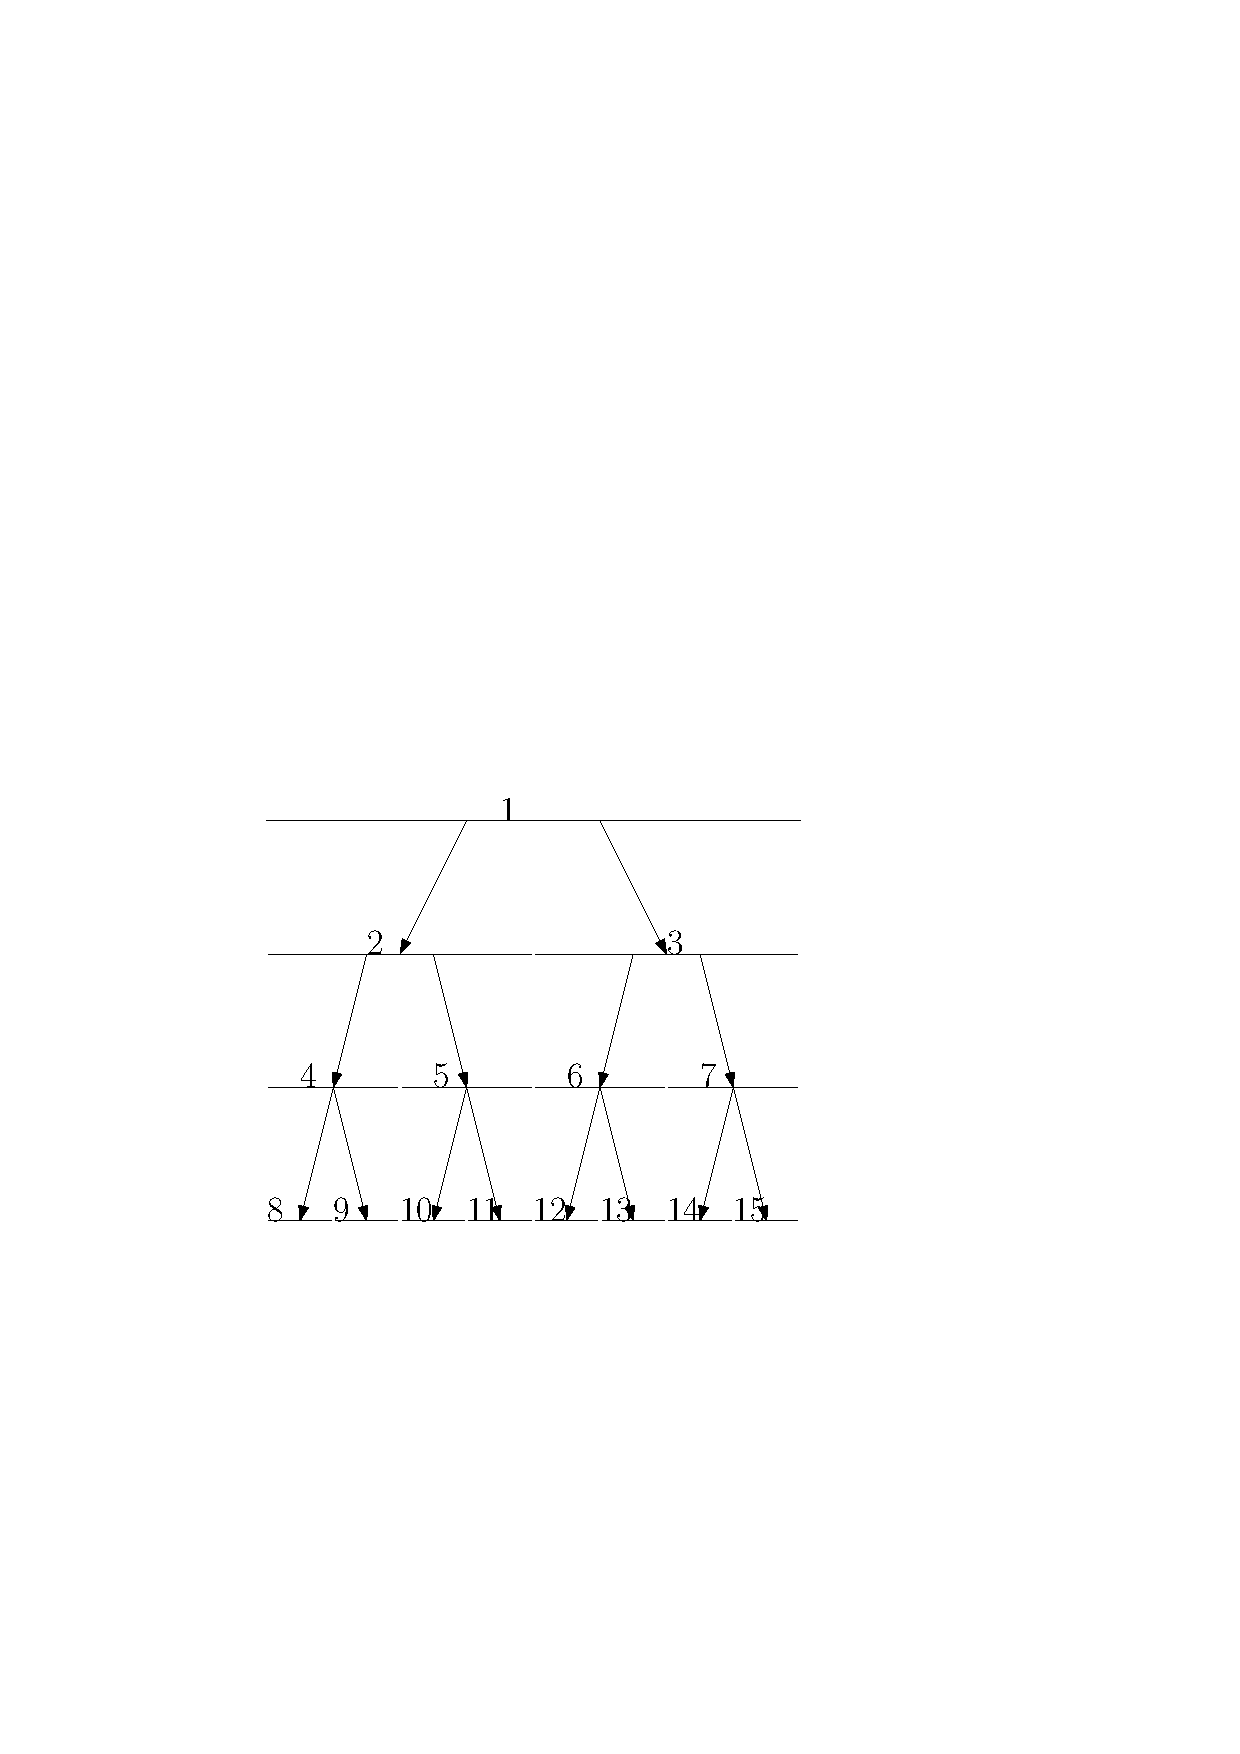
\includegraphics[scale=0.7,page=1]{fig/segtree}
	\caption{The segment tree is a complete or almost complete binary tree.
	Each tree node is associated with an interval.
	The root node represents the total range, and the children of each branch node divide the range of the node into two parts.}\label{fig:segtree}
\end{figure}

The structure of a semi-dynamic segment tree is independent of the intervals stored in the tree.
The nodes are commonly arranged into an almost complete binary tree, which allows storing the tree nodes in an array similarly to binary heap~\cite{kkkk}:
the root node is stored in index~1, and the children of node $i$ are $2i$ and $2i+1$.
This representation allows implementing segment tree operations with very low overhead, making the segment tree a powerful practical tool in addition to providing asymptotical bounds.

\subsection{Canonical nodes}

When an interval $I$ is added to a segment tree, it is stored into several tree nodes called the \emph{canonical nodes} of $I$, denoted by \canon{I}.
The canonical nodes of $I$ are the smallest set of nodes whose intervals cover $I$ but nothing else: $\cup_{c\in\canon{I}} \inter{c}=I$.
Figure~\ref{fig:canon} shows an example of canonical nodes.

\begin{figure}\centering
	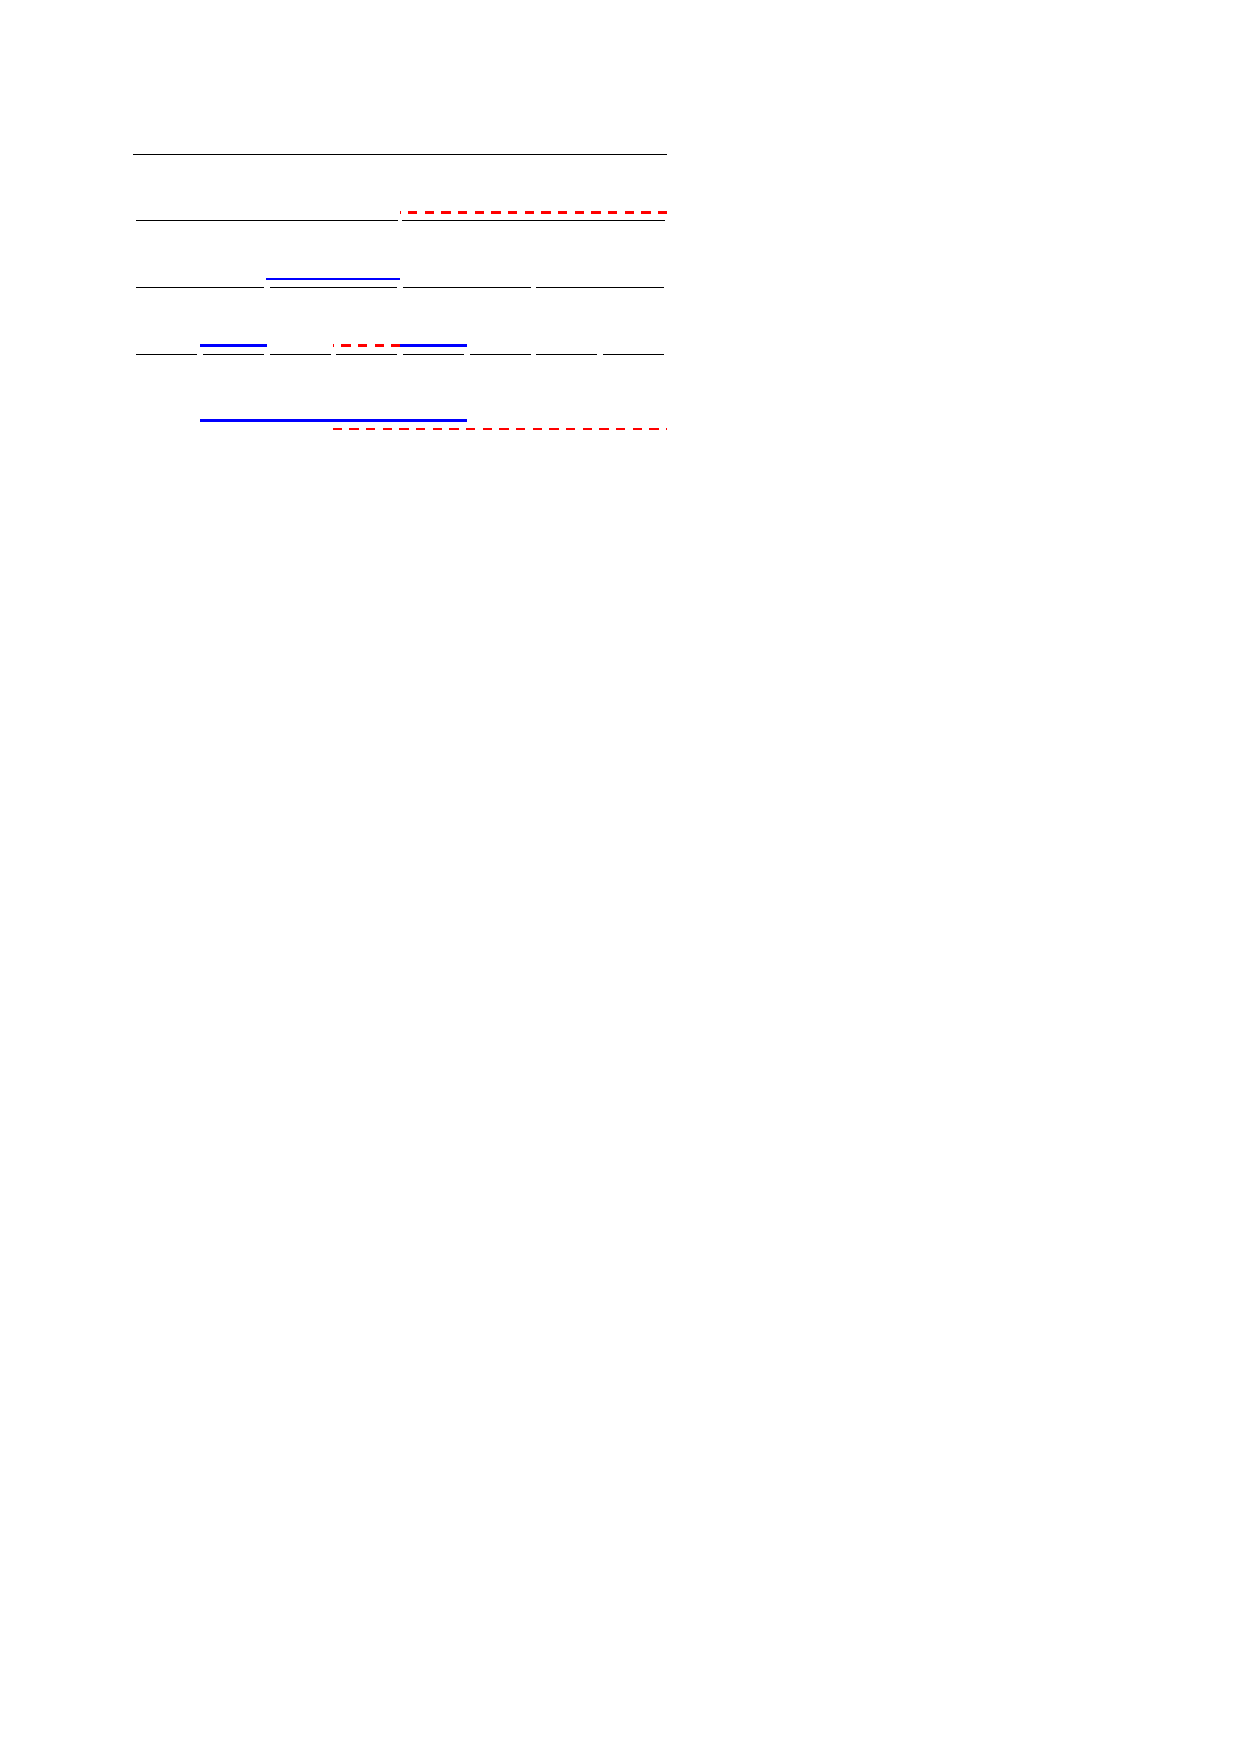
\includegraphics[scale=0.75,page=1]{fig/canon}
	\caption{The canonical nodes of an interval $I$ are the smallest set of nodes covering exactly $I$.
	The number of canonical nodes \canon{I} and their ancestors \canonpar{I} is $O(\log\segsize)$.}\label{fig:canon}
\end{figure}

The set of ancestors of \canon{I} is denoted \canonpar{I}.
The following two lemmas are useful for proving the running times of segment tree operations.

\begin{lem}\label{lem:canonlog}$\size{\canon{I}}=O(\log\segsize)$ for any interval $I$.\end{lem}
\begin{proof}
As the segment tree is a balanced binary tree, it has depth $\Theta(\log\segsize)$.
We show that $\canon{I}$ contains at most 2 nodes on each depth, which proves the claim.

If a set $S$ contains 3 nodes on the same depth, we can replace the middle one with its parent node without affecting the interval covered by $S$.
Thus $S$ is not a minimal cover of $I$, and can not be \canon{I}.
\end{proof}

\begin{lem}\label{lem:canonplog}$\size{\canonpar{I}})=O(\log\segsize)$ for any interval $I$.\end{lem}
\begin{proof}
Similarly to the previous proof we show that \canonpar{I} cannot contain more than 2 nodes on the same depth.

Suppose, for a contradiction, that \canonpar{I} contains 3 nodes on the same depth: $a$, $b$ and $c$ in that order.
Then $\inter{a}\cap I\neq\emptyset$ and $\inter{c}\cap I\neq\emptyset$, so $\inter{b}\subseteq I$.
Some descendant of $b$ belongs to \canon{I}, so \canon{I} is not a minimal cover, which is a contradiction.
\end{proof}

We can iterate over the canonical nodes and their ancestors by using the following recursive algorithm starting from the root node.

\begin{alg}\label{alg:segiter}
Visit all the elements of \canon{I} and \canonpar{I}.
\begin{algorithmic}
\Procedure{IterCanonical}{$s$}
\Comment{Visit the canonical nodes in the subtree rooted at node $s$}
	\If{$\inter{s}\subseteq I$}
		\State $\visitc(s)$.
	\ElsIf{$\inter{s}\cap I\neq\emptyset$}
		\State $\visitp(s)$.
		\State $\textsc{IterCanonical}(\leftc{s})$.
		\State $\textsc{IterCanonical}(\rightc{s})$.
	\EndIf
\EndProcedure
\end{algorithmic}
\end{alg}

Algorithm~\ref{alg:segiter} can be used to implement operations such as adding an interval to a segment tree by defining the methods \visitc and \visitp appropriately.
The recursion traverses through the nodes in \canonpar{I}, and stops immediately when it arrives either to a node in \canon{I} or to a node neither in \canon{I} nor in \canonpar{I}.
Thus the running time is proportional to the sizes of \canon{I} and \canonpar{I}, which is $O(\log\segsize)$ by Lemma~\ref{lem:canonlog} and Lemma~\ref{lem:canonplog}.

\subsection{Tree operations}\label{sec:treeops}

We now show how the segment tree can be used for finding intersecting intervals~\cite[Chapter 10]{berg2008}.
The following lemma gives the necessary and sufficient conditions for detecting intersecting intervals by using the canonical nodes.
Figure~\ref{fig:iproof} illustrates the different cases of the lemma.

\begin{figure}\centering
	\begin{subfigure}[t]{0.32\textwidth}\centering
		\includegraphics[width=\textwidth,page=3]{fig/iproof}
		\caption{$\canon{I}\cap\canon{J}\neq\emptyset$}\label{fig:iproof:common}
	\end{subfigure}
	\hfil
	\begin{subfigure}[t]{0.32\textwidth}\centering
		\includegraphics[width=\textwidth,page=4]{fig/iproof}
		\caption{$\canon{I}\cap\canonpar{J}\neq\emptyset$}\label{fig:iproof:anc}
	\end{subfigure}
	\hfil
	\begin{subfigure}[t]{0.32\textwidth}\centering
		\includegraphics[width=\textwidth,page=2]{fig/iproof}
		\caption{$I\cap J=\emptyset$}\label{fig:iproof:no}
	\end{subfigure}
	\caption{Different cases of Lemma~\ref{lem:segintersect}.
	If a pair of intervals intersect, they either have a common canonical node (Fig.~\ref{fig:iproof:common}) or an ancestor of a canonical node of one interval is a canonical node of the other interval (Fig.~\ref{fig:iproof:anc}).
	If the intervals don't intersect, the canonical sets are also separate (Fig.~\ref{fig:iproof:no}).}\label{fig:iproof}
\end{figure}

\begin{lem}\label{lem:segintersect}Consider any two intervals $I$ and $J$.
At least one of the following is true if and only if $I\cap J\neq\emptyset$.
\begin{enumerate}
\item $\canon{I}\cap\canon{J}\neq\emptyset$,
\item $\canon{I}\cap\canonpar{J}\neq\emptyset$,
\item $\canonpar{I}\cap\canon{J}\neq\emptyset$.
\end{enumerate}
\end{lem}
\begin{proof}
First suppose that $I\cap J\neq\emptyset$.
Let $x$ be any leaf node of the segment tree such that $\inter{x}\in I\cap J$.
Let $A$ be the set of ancestors of $x$.
Since the canonical nodes of an interval cover the whole interval, $A$ intersects both \canon{I} and \canon{J}.
Let $i$ and $j$ be the nodes where $A$ intersects \canon{I} and \canon{J} respectively.
Either $i$ and $j$ are the same node, or one of them is an ancestor of the other, which proves the "if" part of the claim.

For the "only if" part, we look at the three cases separately.
\begin{enumerate}
\item If there exists a node $s\in\canon{I}\cap\canon{J}$, then $\inter{s}\subseteq I\cap J$, so $I\cap J\neq\emptyset$.
\item If there is a node $s\in\canon{I}\cap\canonpar{J}$, then there exists $m\in\canon{J}$ that is a descendant of $s$. $\inter{m}\subseteq J$ and $\inter{m}\subsetneq\inter{s}\subseteq I$, so $I\cap J\neq\emptyset$.
\item Identical to the second case.
\end{enumerate}
\end{proof}

Lemma~\ref{lem:segintersect} can be used to find intersecting pairs of intervals in a segment tree.
In each node $s$ of the segment tree, maintain two lists of intervals:
\begin{itemize}
\item \nodecs{s}: Intervals $I$ for which $s\in\canon{I}$,
\item \nodeps{s}: Intervals $I$ for which $s\in\canonpar{I}$.
\end{itemize}
When an interval $I$ is added to the segment tree, it is added to \nodecs{s} for all $s\in\canon{I}$ and to \nodeps{s} for all $s\in\canonpar{I}$.
When we look for intervals intersecting a given interval $J$, we report all the intervals in \nodecs{s} for all $s\in\canonpar{J}$ and in \nodeps{s} for all $s\in\canon{J}$.
By Lemma~\ref{lem:segintersect} this finds exactly the intervals intersecting $J$ and nothing else.
Note, though, that some intervals might be counted multiple times.
The structure can be further extended to avoid reporting the duplicates, but for the minimum link paths use case we only need to check whether the intersecting set is empty, so this solution is sufficient.

We also want to support clearing an interval from the tree.
Clearing an interval $I$ means that all the intervals $J$ in the tree are cut into $J\setminus I$, potentially removing $J$ or cutting it into two parts.
The clear operation is performed in the following three steps:
\begin{enumerate}
\item Push down the intervals stored in each $s\in\canonpar{I}$ into \leftc{s} and \rightc{s}.
\item Clear each subtree rooted in any node $s\in\canon{I}$.
\item Recompute \nodeps{s} to match the remaining nodes for all nodes $s\in\canonpar{I}$.
\end{enumerate}

All the tree operations can be done in parallel during a single recursive traversal of the tree.
For nodes $s\in\canonpar{I}$ we push down the intervals in \nodecs{s} to the child nodes before proceeding with the recursion.
When we arrive in a node $s\in\canon{I}$, the entire subtree rooted at $s$ is cleared.
After the child nodes are cleared, we also need to regenerate the \nodeps{s} list for the nodes $s\in\canonpar{I}$ to remove the intervals that are no longer present in the subtree.
The regeneration is done by merging the lists in the child nodes of $s$.
The exact algorithm for clearing is shown below.

\begin{alg}\label{alg:segrm}
Clear interval $I$ from a segment tree.
\begin{algorithmic}
\Procedure{ClearInterval}{$s$}
	\Comment Clears interval $I$ from subtree rooted at $s$.
	\If{$\inter{s}\cap I=\emptyset$ or (\nodeps{s} and \nodecs{s} are empty)}
		\State Return.
	\EndIf
	\If{$\inter{s}\nsubseteq I$}
		\State Copy \nodecs{s} to \nodecs{\leftc{s}} and to \nodecs{\rightc{s}}.
	\EndIf
	\State Clear \nodecs{s}.
	\State Clear \nodeps{s}.
	\If{\leftc{s} and \rightc{s} are defined}
		\State $\cleariv(\leftc{s})$.
		\State $\cleariv(\rightc{s})$.
	\EndIf
	\If{$\inter{s}\nsubseteq I$}
		\State $\nodeps{s}\gets \nodeps{\leftc{s}} \cup \nodeps{\rightc{s}} \cup \nodecs{\leftc{s}} \cup \nodecs{\rightc{s}}$.
	\EndIf
\EndProcedure
\end{algorithmic}
\end{alg}

The running time of Algorithm~\ref{alg:segrm} depends on the time taken for copying and merging the intervals stored in the tree nodes.
If we are only interested in querying whether a given interval overlaps any interval in the tree rather than finding the overlapping intervals, we can replace the interval lists by booleans indicating whether the list is empty.
We analyze this more simple case.

\begin{lem}\label{lem:segrmtime}Suppose that the copying and merging of interval sets in Algorithm~\ref{alg:segrm} can be done in constant time.
Then the time complexity of clearing range $I$ is $O(\log\segsize + k)$, where $k$ is the number of cleared nodes.\end{lem}
\begin{proof}
The function \cleariv traverses through nodes \canon{I}, \canonpar{I}, and the descendants of the canonical nodes, stopping immediately if it ends up in an empty subtree.
In each descendant node we either clear the node or return immediately, so we only visit as many descendants as there are cleared nodes.
The number of canonical nodes and their ancestors is $O(\log\segsize)$, so the total time complexity is $O(\log\segsize + k)$.
\end{proof}


\subsection{Multidimensional segment tree}

The segment tree can be generalized into two or higher dimensional structure~\cite{highseg}.
A two-dimensional segment tree allows storing rectangles and performing efficient queries for rectangular regions.
Correspondingly a $D$-dimensional segment tree allows performing efficient operations for $D$-dimensional hyperrectangles.
We use the terms rectangle and hyperrectangle interchangeably to refer to hyperrectangles of any dimension $D$.

A multidimensional segment tree is composed of of nested regular segment trees.
The shape of a $D$-dimensional segment tree is a 1-dimensional segment tree whose each node stores a $(D-1)$-dimensional segment tree.

Each tree dimension represents one of the $D$ coordinate axes.
Each node $s$ of the innermost segment tree represents a $D$-dimensional hyperrectangle \rect{s}, whose bounds are defined by the position of the node in each of the $D$ tree layers.
For example the outer tree of a 2-dimensional segment tree represents the $y$ coordinates, and each inner tree represents the $x$ coordinates.
Each node of the inner tree represents a rectangle whose $x$-bounds are determined by the position of the node in the inner tree, and the $y$-bounds are determined by the node of the outer tree that contains the inner tree.

The concept of canonical nodes can also be extended to higher dimensions~\cite{segbool}.
The canonical nodes \canon{R} of a $D$-dimensional rectangle $R$ are the smallest set of nodes that fully cover $R$ but nothing else.
Figure~\ref{fig:canon2d} illustrates the structure of a 2D segment tree and the canonical nodes.

\begin{figure}\centering
	\begin{subfigure}[t]{0.15\textwidth}\centering
		\includegraphics[width=\textwidth,page=2]{fig/segtree2d}
		\caption{Rectangle $R$ relative to total area}\label{fig:canon2d:r}
	\end{subfigure}
	\hfil
	\begin{subfigure}[t]{0.75\textwidth}\centering
		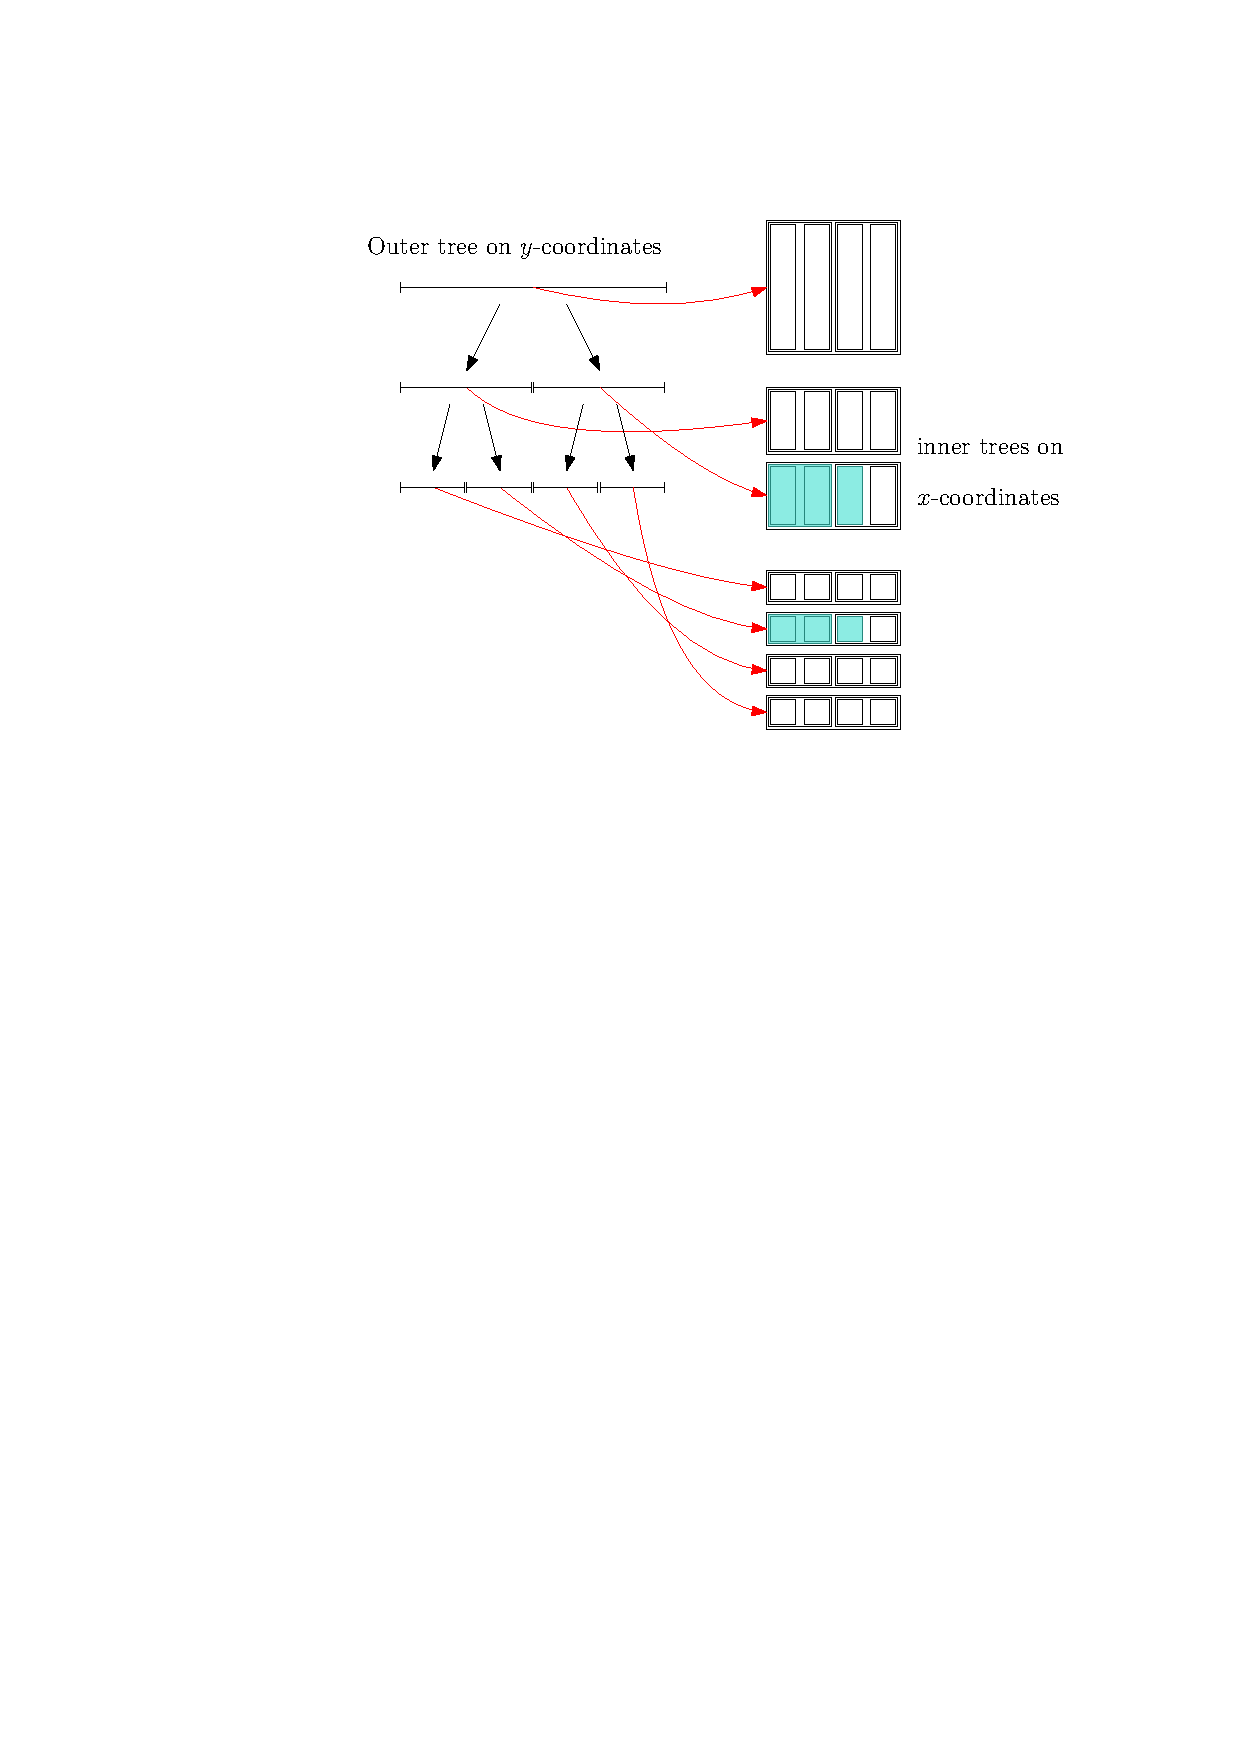
\includegraphics[width=\textwidth,page=1]{fig/segtree2d}
		\caption{The canonical nodes of $R$ in a 2D segment tree}\label{fig:canon2d:tree}
	\end{subfigure}
	\caption{Each node of the outer tree defines a range of $y$-coordinates and an inner segment tree built on $x$-coordinates.
	Each node of the inner trees is a rectangle that combines the $y$ and the $x$ ranges.
	The canonical nodes of a rectangle $R$ (Fig.~\ref{fig:canon2d:r}) are the smallest set of nodes of the inner trees that cover exactly $R$ (Fig.~\ref{fig:canon2d:tree}).}\label{fig:canon2d}
\end{figure}

In order to compute the canonical nodes we look into each axis separately.
Let interval $R_i$ be the projection of rectangle $R$ into $i$-axis.
Let $\canoni{R_i}{i}$ be the canonical rectangles of $R_i$ in the 1-dimensional segment tree built for $i$-coordinates.

Consider a 2-dimensional segment tree, and two arbitrary nodes of the projected 1-dimensional trees $c_1\in\canoni{R_1}{1}$ and $c_2\in\canoni{R_2}{2}$.
Let $c_1\times c_2$ be the node of the 2-dimensional tree that is found in position of $c_1$ in the inner tree, and $c_2$ in the outer tree.
Similarly for $D$-dimensional trees we define product $c_1\times c_2\times\dots\times c_n$ to be the node of a $D$-dimensional segment tree defined by positions of 1-dimensional tree nodes.
The following lemma shows how the canonical nodes of 1-dimensional projections can be combined to get the canonical nodes of a $D$-dimensional tree.

\begin{lem}\label{lem:canond}
For any $D$-dimensional rectangle $R$ applies
$$\canon{R}=\set{c_1\times c_2\dots\times c_D \mid c_1\in\canoni{R_1}{1}, \dots, c_D\in\canoni{R_D}{D}}.$$
In other words, \canon{R} is the Cartesian product of one-dimensional canonical sets
$$\canon{R}=\bigtimes_{i=1}^D \canoni{R_i}{i}.$$
\end{lem}
\begin{proof}
Proof by induction on $D$.
The base case $D=1$ follows directly from the definition of \canon{R}.

For $D\ge 2$ note that all of the inner $(D-1)$-dimensional segment trees are identical.
Thus to cover a rectangular region minimally, we should select the same set of nodes in each inner tree.
By induction we should select the nodes $\bigtimes_{i=1}^{D-1} \canoni{R_i}{i}$ in the inner trees to cover axes $1\dots D-1$ optimally.
To cover also axis $D$, it is optimal to select the nodes $\canoni{R_D}{D}$, and thus $\canon{R}=\bigtimes_{i=1}^D\canoni{R_i}{i}$.
\end{proof}

Combination of Lemma~\ref{lem:canond} and Lemma~\ref{lem:canonlog} gives a bound for the number of canonical nodes.

\begin{cor}\label{cor:canondcount}$\size{\canon{R}}=O(\log^D\segsize)$ for any $D$-dimensional rectangle $R$.\end{cor}
\begin{proof}
$$
\size{\canon{R}} = \size{\bigtimes_{i=1}^D \canoni{R_i}{i}}
= \prod_{i=1}^D \size{\canoni{R_i}{i}}
= \prod_{i=1}^D O(\log\segsize)
= O(\log^D\segsize).
$$
\end{proof}

For 1-dimensional segment trees there is a clear connection between the parent-child hierarchy and interval overlap.
For any two tree nodes $a$ and $b$, $\inter{a}\subseteq\inter{b}$ holds if and only if $b$ is an ancestor of $a$ in the tree.
In multidimensional case it also applies that if $b$ is an ancestor of $a$, then $\rect{a}\subseteq\rect{b}$.
However the reverse is not true; $\rect{a}\subseteq\rect{b}$ does not imply that $b$ is an ancestor of $a$ because $b$ can be in a different subtree in some of the outer trees.

Instead of looking for parent-child relationships directly in the tree, we can look at them separately on each coordinate axis.
This allows us to generalize Lemma~\ref{lem:segintersect} for segment interaction to work for $D$-dimensional rectangles.

\begin{lem}\label{lem:rectintersect}Consider any two $D$-dimensional rectangles $A$ and $B$.
If $A\cap B\neq\emptyset$, then at least one of the following holds for each coordinate axis $d\in\set{1,\dots,D}$.
\begin{enumerate}
\item $\canoni{A_d}{d}\cap\canoni{B_d}{d}\neq\emptyset$,
\item $\canoni{A_d}{d}\cap\canonpari{B_d}{d}\neq\emptyset$,
\item $\canonpari{A_d}{d}\cap\canoni{B_d}{d}\neq\emptyset$.
\end{enumerate}
Furthermore, if $A\cap B=\emptyset$, then there is at least one coordinate axis for which none of the above conditions hold.
\end{lem}
\begin{proof}
$A$ and $B$ overlap if and only if their projections to each coordinate axis overlap.
Suppose that $A\cap B\neq\emptyset$.
Then $A_d$ and $B_d$ overlap for each $d$, and by Lemma~\ref{lem:segintersect} the condition holds for each $d$.
If $A\cap B=\emptyset$, then there exists some $d$ for which $A_d\cap B_d=\emptyset$, so again by Lemma~\ref{lem:segintersect} none of the conditions hold for $d$.
\end{proof}

To find pairs of rectangles fulfilling the conditions of Lemma~\ref{lem:rectintersect}, we store \emph{two} $D-1$ dimensional inner trees in every outer node of a $D$-dimensional segment tree:
\begin{description}
\item[\subtree{s}] where we store rectangles $R$ for which $s\in\canoni{R_D}{D}$,
\item[\subtreep{s}] where we store rectangles $R$ for which $s\in\canonpari{R_D}{D}$.
\end{description}

We can implement rectangle insertion and query operations by using these fields.
For simplicity we only support checking whether a query rectangle intersects any rectangle in the tree rather than returning the matching rectangles.
The nodes $s$ of the innermost tree have dimension 0, and they contain only a single boolean \hasrect{s}, which indicates that at least one rectangle is inserted to this subtree.

\begin{alg}\label{alg:rectadd}
Add rectangle $R$ to a $D$-dimensional segment tree.
\begin{algorithmic}
\Procedure{InsertToTree}{$D,s$}
\Comment{Insert to the subtree rooted at node $s$}
	\If{$D=0$}
		\State $\hasrect{s}\gets\texttt{true}$.
	\ElsIf{$\inter{s}\subseteq R_D$}
		\State $\adddt(D-1,\subtree{s})$.
	\ElsIf{$\inter{s}\cap R_D\neq\emptyset$}
		\State $\adddt(D-1,\subtreep{s})$.
		\State $\adddt(D,\leftc{s})$.
		\State $\adddt(D,\rightc{s})$.
	\EndIf
\EndProcedure
\end{algorithmic}
\end{alg}

\begin{alg}\label{alg:rectcheck}
Query whether rectangle $R$ intersects with any rectangle in the $D$-dimensional segment tree.
\begin{algorithmic}
\Procedure{QueryTree}{$D,s$}
\Comment{Check subtree rooted at node $s$}
	\State $R\gets\texttt{false}$.
	\If{$D=0$}
		\State $R\gets\hasrect{s}$.
	\ElsIf{$\inter{s}\subseteq R_D$}
		\State $R\gets \checkdt(D-1,\subtree{s})$.
		\State $R\gets R$ or $\checkdt(D-1,\subtreep{s})$.
	\ElsIf{$\inter{s}\cap R_D\neq\emptyset$}
		\State $R\gets \checkdt(D-1,\subtree{s})$.
		\State $R\gets R$ or $\checkdt(D,\leftc{s})$.
		\State $R\gets R$ or $\checkdt(D,\rightc{s})$.
	\EndIf
	\State Return $R$.
\EndProcedure
\end{algorithmic}
\end{alg}

\begin{lem}\adddt and \checkdt both have time complexity $O(\log^D\segsize)$.\end{lem}
\begin{proof}
Proof by induction on $D$.
For the base case $D=0$ both algorithm finishes in constant time.
For $D\ge 1$, algorithms iterate over the canonical nodes and their ancestors in the outer tree, making $\log\segsize$ calls to the inner trees.
By induction the inner tree operations are done in $O(\log^{D-1}\segsize)$ time, so the total time complexity is $O(\log^D\segsize)$.
\end{proof}

Note that \subtree{} and \subtreep{} are used in opposite ways in the two operations.
In \adddt{} we recurse down to \subtree{} for canonical nodes, and to \subtreep{} for their ancestors, whereas in \checkdt{} we recurse to \subtree{} in the ancestor nodes, and to both of the trees in the canonical nodes.
This allows us to ensure that \adddt{} and \checkdt{} arrive in the same node exactly in the case where the conditions of Lemma~\ref{lem:rectintersect} are fulfilled.

Suppose we first add rectangle $A$ and then query for rectangle $B$ in the tree.
The \checkdt operation returns true if the two operations end up in any common dimension~0 node.
The only way the two operations end up in a common node is if in each dimension $d$ we are in a canonical node of at least one of $A_d$ and $B_d$, and in either a canonical node or in an ancestor of a canonical node for the other rectangle.

Thus we can efficiently support inserting and querying for $D$-dimensional rectangles by a nested structure consisting of multiple levels of segment trees.
However clearing a rectangle in this structure is a more complex operation.
To make the clear operation more simple, we turn into another variant of the multidimensional segment tree, the unified segment tree.

\subsection{Unified segment tree}\label{sec:unifiedtree}

The structure of a multidimensional segment tree depends on how we order the coordinate axes.
For example a two-dimensional segment tree can have either the outer tree represent $y$-coordinates and each inner tree represent $x$-coordinates, or the other way round.
The structure and the parent-child relationships are different in the two cases, but the set of rectangles represented by the nodes of all the inner trees is exactly the same regardless of the order.

The \emph{unified segment tree}, developed by Wagner~\cite{unified}, combines the parent-child links of the different multidimensional segment trees into a single structure.
The unified segment tree is actually not a tree, but a directed graph.
Each node $s$ of the graph represents a $D$-dimensional hyperrectangle.
For each axis $i$ where \rect{s} is not minimal, $s$ has links to two child nodes that divide \rect{s} into two parts along hyperplane perpendicular to $i$-axis.
Thus each node has between 0 and $2D$ links to child nodes.
The children splitting the node $s$ along axis $i$ are denoted by \leftu{s}{i} and \rightu{s}{i}.
Figure~\ref{fig:unified} illustrates the structure of the unified segment tree in 2-dimensional case.

\begin{figure}\centering
	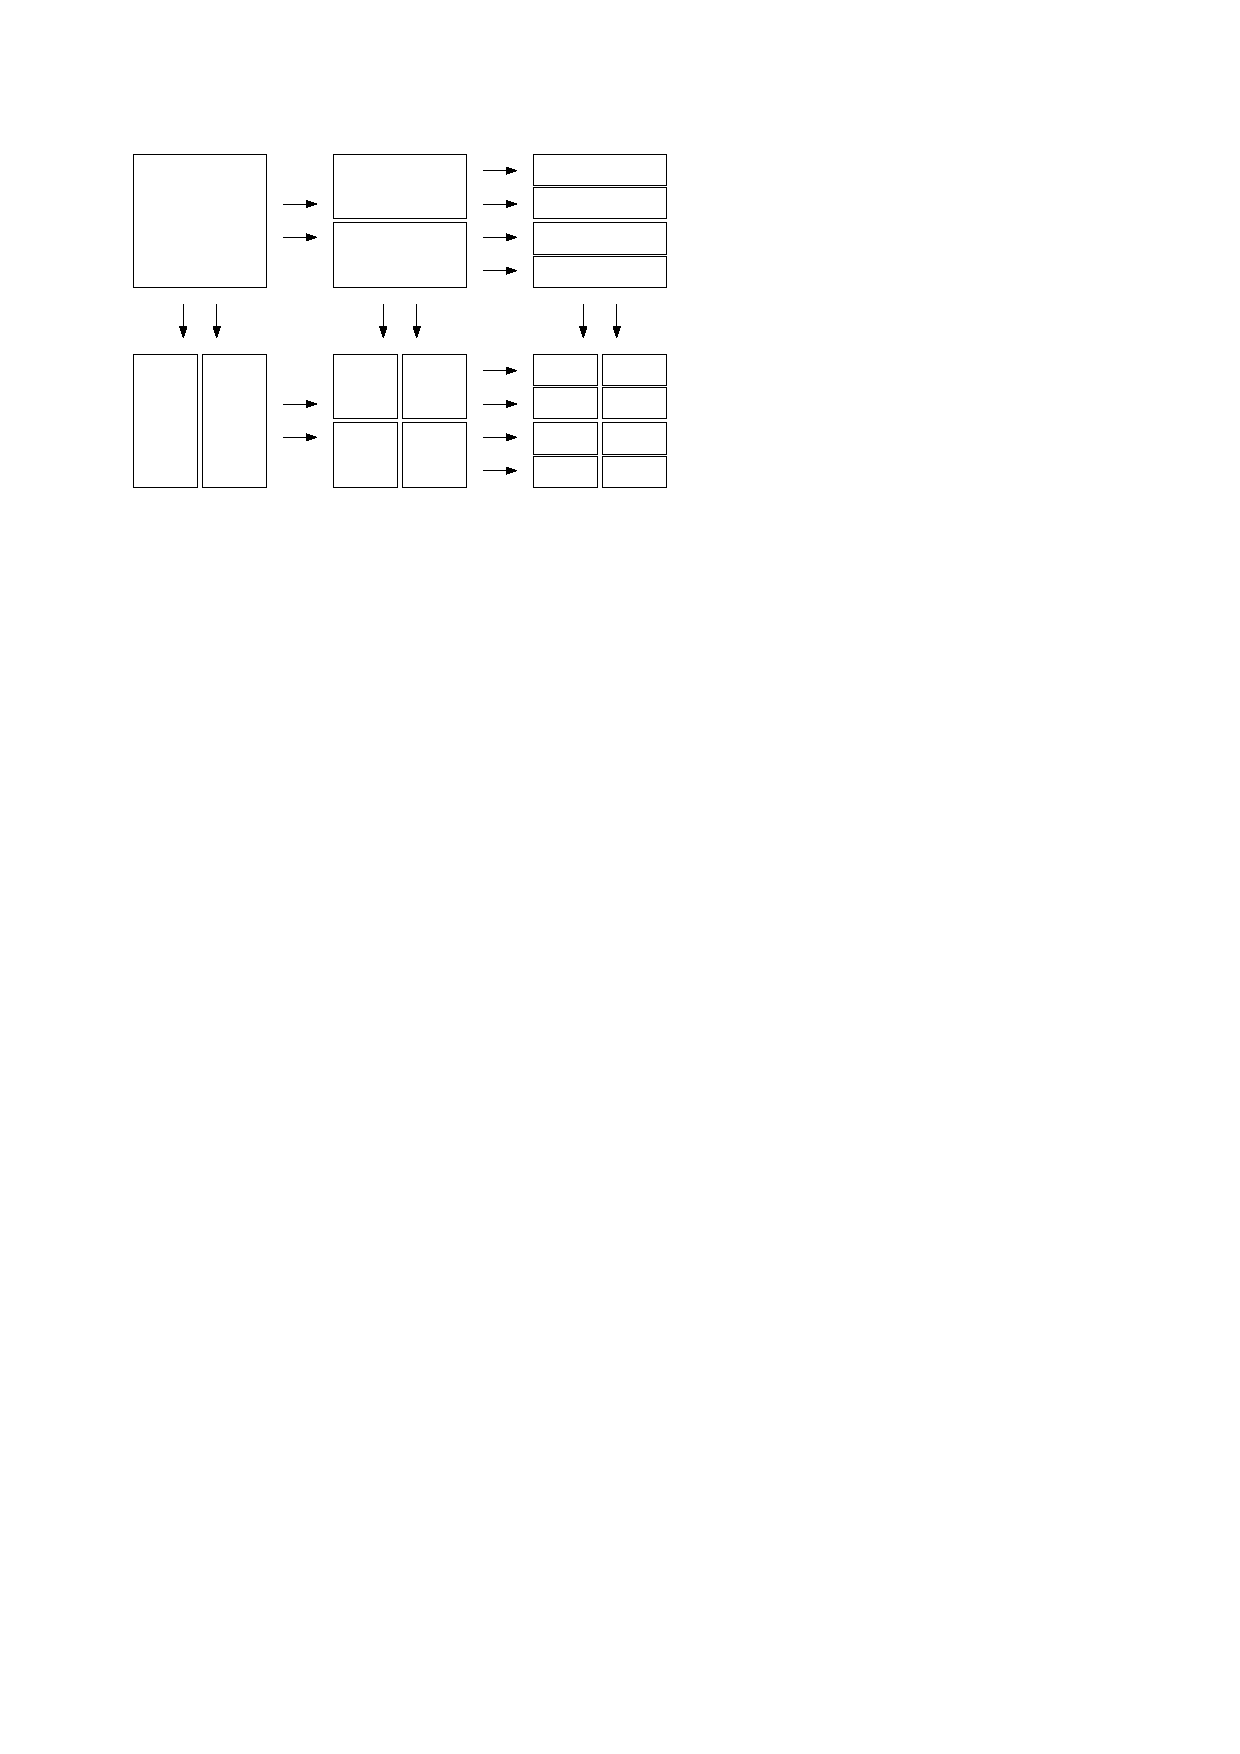
\includegraphics[width=0.5\textwidth]{fig/unified}
	\caption{The nodes of the unified segment tree form a directed acyclic graph.
	Each node can be split along any of the coordinate axes as long as the node is not minimal in that direction.}\label{fig:unified}
\end{figure}

Note that in the unified tree there is no distinction between outer and inner tree.
In the regular multidimensional segment tree the nodes of nested tree represent ranges in one of the coordinate axes, and the innermost nodes represent their Cartesian product.
In the unified tree there is no concept of outer and inner nodes, and each node represents a $D$-dimensional rectangle.

The operations \adddt and \checkdt for the unified tree are largely similar to the algorithms for the regular multidimensional tree.
We consider again checking whether the query rectangle intersects with any of the rectangles in the tree.
Each tree node stores $2^D$ bits of information about the rectangles stored in the subtree.
The bit array stored in node $s$ is denoted \hasbita{s}.
When a rectangle $R$ is added to node $s$, the bits are used to define whether $s$ represents a canonical node or an ancestor of a canonical node along each coordinate axis.
The $2^D$ bits allow us to detect when the conditions of Lemma~\ref{lem:rectintersect} become fulfilled when querying for intersecting rectangles.

The following function computes a bitmask of $s$ bits for a rectangle and a tree node.
This bits are used to determine which bits of \hasbita{s} to access when adding a rectangle or querying the tree.

\begin{alg}\label{alg:maskof}
Compute bitmask representing whether node $s$ is covered by rectangle $R$ in each direction.
\begin{algorithmic}
\Procedure{NodeMask}{$R,s$}
	\State $m\gets 0$.
	\ForAll{$d \in 1\dots D$}
		\If{$\rect{s}_d\subseteq R_d$}
			\State $m\gets m | 2^{d-1}$.
		\EndIf
	\EndFor
	\State Return $m$.
\EndProcedure
\end{algorithmic}
\end{alg}

We can implement procedures \adddt and \checkdt by using the bitmasks returned by \maskof{}.

\begin{alg}\label{alg:uadd}
Add rectangle $R$ to $D$-dimensional unified tree.
\begin{algorithmic}
\Procedure{InsertToTree}{$d,s$}
\Comment{Insert to the subtree rooted at node $s$ by moving along axes $1\dots d$}
	\If{$d=0$}
		\State $m\gets\maskof{R,s}$.
		\ForAll{$b \in 0\dots 2^D-1$}
			\If{All bits of $b$ are set in $m$}
				\State $\hasbits{s}{b}\gets\texttt{true}.$
			\EndIf
		\EndFor
	\ElsIf{$\rect{s}_d\subseteq R_d$}
		\State $\adddt(d-1,s)$.
	\ElsIf{$\rect{s}_d\cap R_d\neq\emptyset$}
		\State $\adddt(d-1,s)$.
		\State $\adddt(d,\leftu{s}{d})$.
		\State $\adddt(d,\rightu{s}{d})$.
	\EndIf
\EndProcedure
\end{algorithmic}
\end{alg}

For \checkdt we use function $\texttt{reverseBits}$, which reverses the bits of a $2^D$-bit input.
For example if $D=2$ then $\texttt{reverseBits}(0111_2)=1000_2$.

\begin{alg}\label{alg:ucheck}
Query whether rectangle $R$ intersects with any rectangle in the unified tree.
\begin{algorithmic}
\Procedure{QueryTree}{$d,s$}
\Comment{Check subtree rooted at node $s$}
	\State $R\gets\texttt{false}$.
	\If{$d=0$}
		\State $R\gets\hasbits{s}{\texttt{reverseBits}(\maskof{R,s})}$.
	\ElsIf{$\rect{s}_d\subseteq R_d$}
		\State $R\gets\checkdt(d-1,s)$.
	\ElsIf{$\rect{s}_d\cap R_d\neq\emptyset$}
		\State $R\gets\checkdt(d-1,s)$.
		\State $R\gets R$ or $\checkdt(d,\leftu{s}{d})$.
		\State $R\gets R$ or $\checkdt(d,\rightu{s}{d})$.
	\EndIf
	\State Return $R$.
\EndProcedure
\end{algorithmic}
\end{alg}

Both \adddt and \checkdt iterate over the canonical nodes of the input rectangle as well as their ancestors, and access \hasbita{s} for each such node $s$.
When adding a rectangle $A$, we set $\hasbits{s}{b}$ for each bitmask $b$ whose bits are contained in $\maskof{A,s}$.
To query for a rectangle $B$, we check the bit $\hasbits{s}{\texttt{reverseBits}(\maskof{B,s})}$ for the accessed nodes $s$.
This expression detects $A$ if $\maskof{A,s}|\maskof{B,s}=2^D-1$, where $x|y$ represents the bitwise OR operation of $x$ and $y$.
This is equivalent to condition that $\rect{s}_d$ is the range of a canonical node of either $R_d$ or $A_d$ or both in each dimension $d$.
This matches the conditions of Lemma~\ref{lem:rectintersect} for rectangle intersection, so the match is returned if and only if $A$ and $B$ intersect.

Next we consider clearing a rectangle from the unified tree.
Clearing a rectangle $R$ means that all the rectangles in the tree are cut such that the region of $R$ becomes empty.
The clear operation is implemented using the same three operations as we used for the 1-dimensional tree in Section~\ref{sec:treeops}:
push down any intervals in the ancestors, clear the subtrees of the canonical nodes, and finally recompute the information about rectangles stored in the descendants.

The three operations are performed by a recursive function \cleardt that traverses through the tree.
The function uses two arguments to control the tree traversal: the current subtree root $s$, and the axis where we are moving $d$.
In each canonical ancestor $s\in\canonpari{R_d}{d}$ we split the contents of the subtree along axis $d$ before proceeding, and recompute the descendant information after finishing clearing the subtree.
The full algorithm is described below.

\begin{alg}\label{alg:segurm}
Clear rectangle $R$ from $D$-dimensional unified segment tree.
\begin{algorithmic}
\Procedure{ClearFromTree}{$d,s$}
	\If{$\rect{s}_d\cap R_d=\emptyset$ or $\neg\hasbits{s}{0}$}
		\State Return.
	\EndIf
	\If{$d=0$}
		\State $\hasbits{s}{0\dots 2^{D-1}}\gets\texttt{false}$.
		\State Return.
	\EndIf
	\If{$\rect{s}_d\nsubseteq R_d$}
		\State $\pdst(d-1,s,d)$.
	\EndIf
	\State $\cleardt(d-1,s)$.
	\If{\leftu{s}{d} and \rightu{s}{d} are defined}
		\State $\cleardt(d,\leftu{s}{d})$.
		\State $\cleardt(d,\rightu{s}{d})$.
	\EndIf
	\If{$\rect{s}_d\nsubseteq R_d$}
		\State $\recomp(d,s)$.
	\EndIf
\EndProcedure

\Procedure{PushDownSubtree}{$d,s,a$}
	\Comment Pushes down values in subtree $s$ along axis $a$.
	\If{$d=0$}
		\State $\hasbita{\leftu{s}{a}}\gets \hasbita{\leftu{s}{a}} | \hasbita{s}$.
		\State $\hasbita{\rightu{s}{a}}\gets \hasbita{\rightu{s}{a}} | \hasbita{s}$.
		\State Return.
	\ElsIf{$\rect{s}_d\cap R_d=\emptyset$}
		\State Return.
	\EndIf
	\State $\pdst(d-1,s,a)$.
	\If{\leftu{s}{d} and \rightu{s}{d} are defined}
		\State $\pdst(d,\leftu{s}{d},a)$.
		\State $\pdst(d,\rightu{s}{d},a)$.
	\EndIf
\EndProcedure

\Procedure{RecomputeSubtreeData}{$d,s$}
	\If{$d=0$}
		\State $\textsc{RecomputeSubtreeDataForNode}(s)$.
		\State Return.
	\ElsIf{$\rect{s}_d\cap R_d=\emptyset$}
		\State Return.
	\EndIf
	\State $\recomp(d-1,s)$.
	\If{\leftu{s}{d} and \rightu{s}{d} are defined}
		\State $\recomp(d,\leftu{s}{d})$.
		\State $\recomp(d,\rightu{s}{d})$.
	\EndIf
\EndProcedure

\Procedure{RecomputeSubtreeDataForNode}{$s$}
	\State $\hasbita{s}\gets\texttt{false}$.
	\State $m\gets\maskof{R,s}$.
	\ForAll{$a \in 1\dots D$}
		\If{$\rect{s}_a \subseteq R_a$}
			\State Continue.
		\EndIf
		\State $c_1\gets\leftu{s}{a}$.
		\State $c_2\gets\rightu{s}{a}$.
		\ForAll{$b \in 0 \dots 2^D-1$}
			\If{$b$ does not have bit $a$ set}
				\State $\hasbits{s}{b}\gets \hasbits{s}{b}$ or $\hasbits{c_1}{b}$ or $\hasbits{c_2}{b}$.
			\EndIf
		\EndFor
	\EndFor
\EndProcedure
\end{algorithmic}
\end{alg}

\begin{lem}\label{lem:segurmtime}Algorithm~\ref{alg:segurm} has running time $O(\segsize^{D-1}\log\segsize + k)$, where $k$ is the number of cleared canonical nodes.\end{lem}
\begin{proof}
We start by proving that \pdst and \recomp have running time $O(\segsize^d)$ by induction on the argument $d$.
Clearly both functions perform $O(1)$ work when $d=0$, which proves the base case.
If $d\ge 1$, both functions recursively iterate over the descendants in direction $d$, making $O(\segsize)$ recursive calls with argument $d-1$.
By induction the recursive calls are done in $O(\segsize^{d-1})$ time, so the time complexity of both \pdst and \recomp is $O(\segsize^d)$.

Next we prove the running time of \cleardt by induction on argument $d$.
When called with argument $d$, function \cleardt calls functions \pdst and \recomp with argument $d-1$.
If $d=1$ the calls to \pdst and \recomp perform $O(1)$ work, and the algorithm is equivalent to Algorithm~\ref{alg:segrm} for 1-dimensional segment tree removal.
Thus the base case $d=1$ is proven by Lemma~\ref{lem:segrmtime}.

In case $d\ge 2$ we iterate over the descendants in direction $d$.
We call \pdst and \recomp with argument $d-1$ for every node in \canonpari{R_d}{d}.
We also make $O(\segsize)$ calls to \cleardt with argument $d-1$.
The size of \canonpari{R_d}{d} is $O(\log\segsize)$, so by induction the total time complexity is $O((\log\segsize)\segsize^{d-1} + \segsize(\segsize^{d-2}\log\segsize))=O(\segsize^{d-1}\log\segsize)$.
\end{proof}



\section{Minimum link paths in plane}\label{sec:minlink2d}

In this section we study the rectilinear minimum link path problem in plane.
We present a simple algorithm with time complexity $O(n\log n)$ and space complexity $O(n)$~\cite{revisited}.
The ideas developed for the planar case are later generalized to solve the more difficult 3D and higher dimensional minimum link path problems in Section~\ref{sec:minlink3d}.

\subsection{Intersection graph}

We solve the minimum link path problem by applying the staged illumination paradigm outlined in Section~\ref{sec:overview}.
We initialize \reach{0} to contain the starting point~\spt, and iteratively expand the illuminated area by computing \reach{k+1} based on \reach{k}.
The iteration is continued until we find the endpoint~\ept.

Clearly any minimum link path consists of alternation between horizontal and vertical links.
We split the problem into two subproblems, based on whether the first link is horizontal or vertical.
The minimum link path can be found by solving both subproblems and choosing the shorter of the two solutions.

Consider the case with the first link horizontal.
It is easy to see that \reach{k+1} consists of points that can be reached by starting from \reach{k} and moving either horizontally or vertically, depending on the parity of $k$.
The following lemma shows that the regions illuminated on each step can be expressed by using the horizontal and vertical decompositions defined in Section~\ref{sec:decomp2d}.

\begin{lem}\label{lem:illum2d}
For even $k\ge 2$, the region \reach{k+1} consists of the rectangles $r\in\decomp{x}$ that intersect the region \reach{k}.
For odd $k\ge 3$ the same applies for \decomp{y}.
\end{lem}
\begin{proof}
Let $k\ge 2$ be even.
The region \reach{k} is formed by illuminating in vertical direction from \reach{k-1}.

Let $h$ be any rectangle in $\decomp{x}$ that is at least partially illuminated in \reach{k}.
Since \reach{k} is formed by illuminating vertically from \reach{k-1}, there must be a vertical line passing through $h$ that is contained in \reach{k}.
Illuminating horizontally from the vertical line illuminates $h$ entirely, so $h\subseteq\reach{k+1}$.
Thus each rectangle of \decomp{x} intersected by \reach{k} is entirely contained in \reach{k+1}.

For odd $k\ge 3$ we form \reach{k+1} by illuminating in vertical direction from \reach{k}, and the same proof applies for \decomp{y}.
\end{proof}

\begin{figure}\centering
	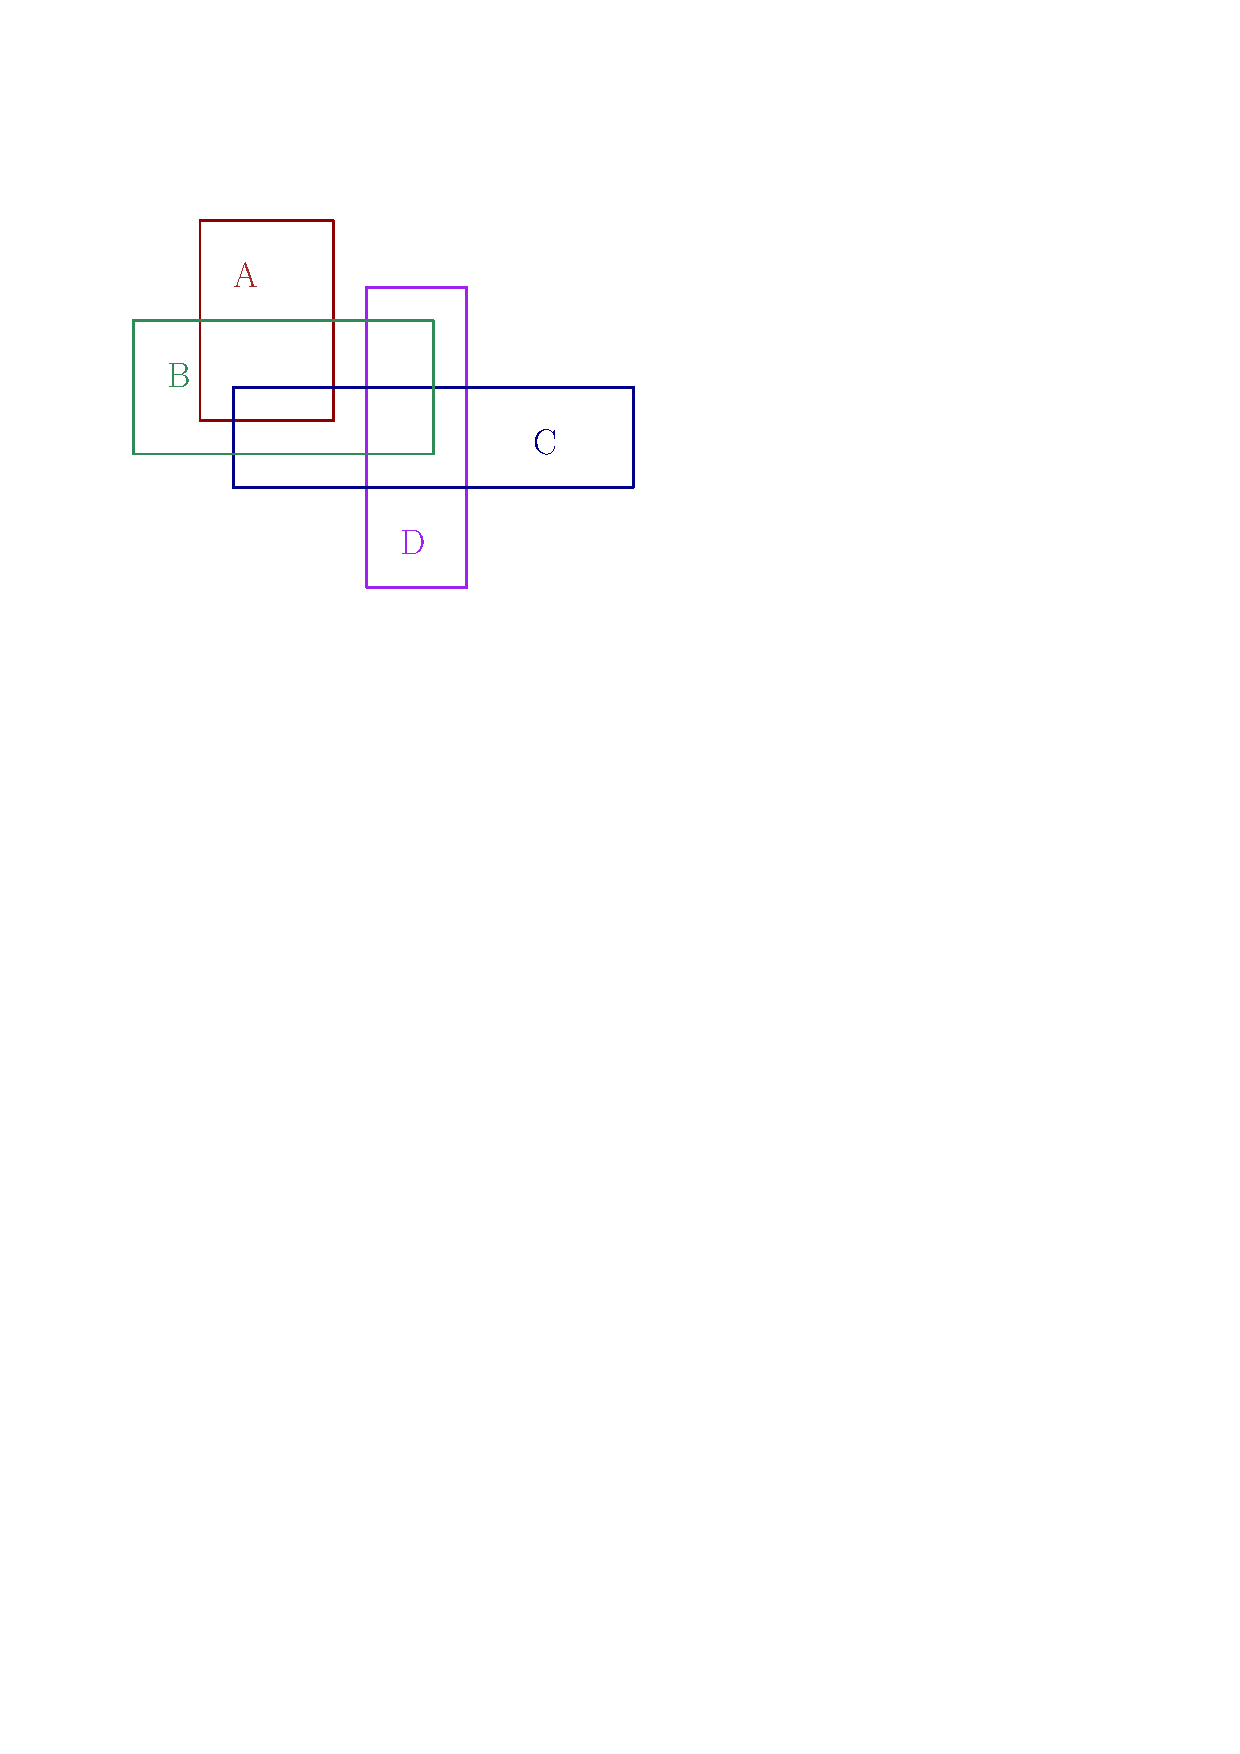
\includegraphics[scale=0.7,page=1]{fig/inter}
	\hfil
	\includegraphics[scale=0.7,page=2]{fig/inter}
	\caption{Group of four rectangles and their intersection graph. Each pair of overlapping objects has an edge between them in the intersection graph.}\label{fig:inter}
\end{figure}

For a set of geometric objects (such as rectangles) $G$, the \emph{intersection graph} of $G$ is a graph whose nodes are the elements of $G$, and there is an edge between each pair of intersecting objects.
Figure~\ref{fig:inter} shows an example of the intersection graph.
Consider the intersection graph of $\decomp{x}\cup\decomp{y}$.
This graph has rectangles as nodes, and intersecting rectangles between \decomp{x} and \decomp{y} are joined by an edge.
Let $k$ be an even number and $r\in\decomp{x}$ contained in \reach{k}.
Then for each neighbor $b$ of $r$ in the intersection graph applies $b\subseteq\reach{k+1}$ by Lemma~\ref{lem:illum2d}.
In other words, the staged illumination finds the rectangles in the same order as breadth-first search in the intersection graph.

The rectilinear minimum link path problem can thus be solved by forming the intersection graph and searching for the shortest path using breadth-first search~\cite{dasnar}.
However the intersection graph has quadratic size, so building it takes at least quadratic time as well.
The goal is thus to implicitly perform BFS in the intersection graph without explicitly constructing the graph.

\subsection{Searching the intersection graph}

Consider again the case where the first link of the path is horizontal.
We start by constructing the horizontal decomposition with Algorithm~\ref{alg:split2d}.
The vertical decomposition is used implicitly in the analysis, but there is no need to construct it explicitly.

\reach{0} contains the start point~\spt, and \reach{1} is the horizontal line segment passing through \spt.
The path finding algorithm works by alternating between two phases~\cite{revisited}:

\begin{enumerate}
\item For odd $k$, \reach{k} consists of a set of rectangles $R_k\subseteq\decomp{x}$.
	Inspect which obstacles can be reached by a vertical line starting from any point in \reach{k}, and form $\hat{R}_{k+1}=\set{r \mid r\in\decomp{x}, r\cap\reach{k+1}\neq\emptyset}$.
\item For even $k$, we simply set $R_{k+1}=\hat{R}_k$.
	Then $\reach{k+1}=\bigcup_{r\in R_{k+1}}r$ by Lemma~\ref{lem:illum2d}.
\end{enumerate}

\begin{figure}\centering
	\begin{subfigure}[t]{0.15\textwidth}\centering
		\includegraphics[width=\textwidth,page=2]{fig/light2d}
		\caption{Initial state}\label{fig:light2d:start}
	\end{subfigure}
	\hfil
	\begin{subfigure}[t]{0.15\textwidth}\centering
		\includegraphics[width=\textwidth,page=3]{fig/light2d}
		\caption{Sweep up}\label{fig:light2d:up}
	\end{subfigure}
	\hfil
	\begin{subfigure}[t]{0.15\textwidth}\centering
		\includegraphics[width=\textwidth,page=4]{fig/light2d}
		\caption{Sweep down}\label{fig:light2d:down}
	\end{subfigure}
	\hfil
	\begin{subfigure}[t]{0.15\textwidth}\centering
		\includegraphics[width=\textwidth,page=5]{fig/light2d}
		\caption{Select rectangles found by the sweeps}\label{fig:light2d:sel1}
	\end{subfigure}
	\hfil
	\begin{subfigure}[t]{0.15\textwidth}\centering
		\includegraphics[width=\textwidth,page=6]{fig/light2d}
		\caption{Sweep up and down}\label{fig:light2d:updown}
	\end{subfigure}
	\hfil
	\begin{subfigure}[t]{0.15\textwidth}\centering
		\includegraphics[width=\textwidth,page=7]{fig/light2d}
		\caption{Select rectangles found by the sweeps}\label{fig:light2d:sel2}
	\end{subfigure}
	\caption{The staged illumination proceeds from starting state (Fig.~\ref{fig:light2d:start}) by iterating two phases:
	1. Illuminate up and down (Fig.~\ref{fig:light2d:up},~\ref{fig:light2d:down},~\ref{fig:light2d:updown}).
	2. Select illuminated rectangles (Fig.~\ref{fig:light2d:sel1},~\ref{fig:light2d:sel2}).
	}\label{fig:light2d}
\end{figure}

We keep iterating the two phases until the endpoint~\ept is reached in either phase.
Figure~\ref{fig:light2d} shows the illumination process.

For performance, it is important to ensure that we don't reilluminate the same parts of the domain many times.
We avoid the reillumination by marking cells of \decomp{x} as obstacles some time after they have been found.
If rectangle $r$ is discovered on step $k$, then it is fully illuminated in \reach{k+1}, and each point visible from $r$ is illuminated in \reach{k+2}.
After this there is no longer any need to illuminate through $r$, so we can treat $r$ as an obstacle after 2 steps have passed since the illumination first reached $k$.
This ensures that each rectangle is illuminated only a constant number of times.

Next we show how to implement illumination in $y$-direction starting from \reach{k}, which is represented as a set of rectangles $R\in\subseteq\decomp{x}$.
The illuminated area is computed with two line sweeps, in in direction $+y$ and the other in direction $-y$.

The sweep line stops at each rectangle to be illuminated.
During the sweep we maintain the intersection between the sweep line and the newly illuminated region \reach{k+1}.
The intersection consists of non-overlapping intervals stored in a binary search tree.

Let \nbsd{r}{d} and \obsd{r}{d} be the neighbor cell and the adjacent obstacles of rectangle $r$ in direction $d$ in \decomp{x}.
The algorithm below describes the illumination in direction $+y$.
The sweep in direction $-y$ is identical.

\begin{alg}\label{alg:light2d}
Compute illuminated rectangles from group $R$ into direction $+y$.
\begin{algorithmic}
\State $Q\gets\text{Priority queue containing the rectangles of $R$, ordered by the highest $y$-coordinate}$.
\State $T\gets\text{Empty binary search tree}$.
\While{$Q$ is not empty}
	\State $r\gets\pop{Q}$.
	\If{$r\in R$}
		\State Insert \xrange{r} into $T$.
	\EndIf
	\ForAll{$o\in\obsd{r}{+y}$}
		\ForAll{$t\in T$ touching \xrange{o}}
			\State Replace $t$ by $t\setminus\xrange{o}$, possibly removing it or splitting it into two parts.
		\EndFor
	\EndFor
	\ForAll{$b\in\nbsd{r}{+y}$}
		\If{$\xrange{b}$ touches any range in $T$ and $b\notin Q$}
			\State Insert $b$ into $Q$.
		\EndIf
	\EndFor
\EndWhile
\end{algorithmic}
\end{alg}

\begin{lem}\label{lem:light2dtime}The running time of Algorithm~\ref{alg:light2d} is $O(m\log m)$ where $m$ is the number of visited rectangles and their neighbor links.\end{lem}
\begin{proof}
The outermost loop processes a different rectangle $r$ each time, so it is executed $O(m)$ times.
For each obstacle adjacent to $r$ we cut of all the intersections with the obstacle from the binary search tree.
At most two of the intersected intervals remain in the tree, the others are removed, so the cost of the clearing operation can be accounted to the point when the nodes where added to the tree.
Thus the cost of processing an obstacle if $O(\log m)$ when the removing time is accounted to the insertions.
For each rectangle adjacent to $r$ we perform a single binary tree operation and possibly a single operation to the binary queue, which can both be done in $O(\log m)$ time.
Thus the total time complexity is $O(m\log m)$.
\end{proof}

The link distance between \spt and \ept can be computed by iteratively performing the illumination sweeps in $+y$ and $-y$ directions until the endpoint is found.

\begin{alg}\label{alg:minlink2d}
Run staged illumination starting from \spt within \fspace such that the first link is horizontal.
\begin{algorithmic}
\State Form \decomp{x} for \fspace with Algorithm~\ref{alg:split2d}.
\State $R\gets\set{r\in\decomp{x} \mid \spt\in r}$
\State $k\gets 1$
\While{$R\neq\emptyset$}
	\ForAll{$r\in R$}
		\If{$\stepof{r}$ is not set}
			\State $\stepof{r}\gets k$
		\ElsIf{$\stepof{r} \le k-2$}
			\State Mark $r$ to be treated as obstacle during the sweeps.
			\State Remove $r$ from $R$.
		\EndIf
	\EndFor
	\State $H_{+y}\gets H$ illuminated in direction $+y$ by Algorithm~\ref{alg:light2d}.
	\State $H_{-y}\gets H$ illuminated in direction $-y$ by Algorithm~\ref{alg:light2d}.
	\State $H\gets H_{+y}\cup H_{-y}$.
	\State $k\gets k+1$
\EndWhile
\end{algorithmic}
\end{alg}

\begin{theo}Algorithm~\ref{alg:minlink2d} has time complexity $O(n\log n)$ and space complexity $O(n)$.\end{theo}
\begin{proof}
\decomp{x} is formed in $O(n\log n)$ time by Lemma~\ref{lem:split2dtime}.
\decomp{x} has $O(n)$ cells and links between cells.
Each cell is marked as an obstacle 2 steps after it has been found.
On each iteration of the main loop we perform two sweeps, so each cell can be visited at most 4 times by the sweeps.
The time complexity of a single sweep is $O(m\log m)$ by Lemma~\ref{lem:light2dtime}, where $m$ is the number of visited rectangles.
Since each rectangle can be visited $O(1)$ times, the total time complexity of all the sweeps is $O(n\log n)$.

The decomposition is created in linear space, and the sweeps only use simple binary search tree and binary heap structures taking linear space, so the whole algorithm runs in $O(n)$ space.
\end{proof}

The link distance between \spt and a target point \ept can be found by stopping the illumination process as soon as \ept becomes illuminated.
\epts can become illuminated either during a vertical sweep, or the implicit horizontal sweep that happens when we assign $H_{+y}\cup H_{-y}$ into $H$.
To construct the minimum link path between \spt and \ept, augment the algorithm such that we store into each rectangle how it was initially illuminated, and trace back the path when \ept gets illuminated.



\section{Paths in three and higher dimensions}\label{sec:minlink3d}

In this section we study the rectilinear minimum link path problem in 3D domain.
We present an algorithm that has time complexity $O(n^2\log^2n)$ and space complexity $O(n^2)$~\cite{restricted}.
We also extend the algorithm to work in higher dimensions.
For any constant $D\ge 2$, the presented algorithm works in $O(n^{D-1}\log^{D-1}n)$ time.

Some of the basic ideas of the 2D minimum link path algorithm can also be applied to the 3D case.
The path is computed using the staged illumination paradigm, and on each step we compute \reach{k+1} from \reach{k} by using sweep plane algorithms in all the coordinate axis directions.
However in 3D case the representation of the illuminated space becomes more complicated, and also the sweep algorithms require more sophisticated logic.

We use the decomposition presented in Section~\ref{sec:split3d} to maintain the illuminated set and to guide the illumination during the sweeps.
Unlike the 2D case, the algorithm does not use any specific properties of the decomposition, but can be used with any space decomposition.
The running time of the algorithm depends on the number of cells and links between them, and the decomposition we use has the advantage of having only a small number of links.

The decomposition is used to implement plane sweep algorithm for computing \reach{k+1} from \reach{k}.
On each step we run 6 sweeps, one in each of the directions $\pm x$, $\pm y$ and $\pm z$.
By combining the results of sweeping in each direction we form the whole region \reach{k+1}.
Next we discuss how the sweep plane algorithm is implemented, and then show how the minimum link path algorithm is built around it.

\subsection{Illumination by plane sweep}

We use a sweep plane algorithm to compute \reach{k+1} from \reach{k}~\cite{restricted}.
The sweep performs two functions: it discovers which cells can be illuminated from \reach{k}, and it constructs the boundary of the illuminated region.
The boundary is used on the next step to compute \reach{k+2} from \reach{k+1}.

During the sweep we maintain the intersection of the sweep plane with the newly illuminated region, and a priority queue of events.
The events belong to one of the following types:

\begin{description}
\item[\addE] where a previously illuminated region is added to the sweep plane.
\item[\cellE] which occurs when the sweep plane reaches the end of a cell that potentially intersects with the illuminated region.
\item[\obsE] which occurs when the sweep plane encounters an obstacle face with normal opposite of the sweep direction.
\end{description}

Suppose that we are performing the sweep in direction $+z$.
In \cellE we first check whether the reached cell $c$ is truly illuminated.
If yes, we add a \cellE for each neighbor of $c$ in direction $+z$, and an \obsE for each obstacle adjacent to $c$ in direction $+z$.
In \obsE the projection of the encountered obstacle is cleared from the sweep plane.
Additionally the cleared rectangles are used to construct new \addEs on the boundary of the illuminated region to be used on the next illumination step.

During the sweep, the intersection of the illuminated region with the sweep plane is stored in the Unified 2D segment tree presented in Section~\ref{sec:unifiedtree}.
Each \addE inserts a new rectangle to the tree.
Each illuminated canonical node of the tree stores reference to the event that was used to generate it.
If multiple \addEs illuminate the same canonical rectangle, only the one inserted first is stored.
This reference is used to determine the $z$-range of the \addEs generated during \obsE, as well as for tracing back the path from \ept to \spt after the illumination is finished.

Pseudocode for the illumination plane sweep is as following.

\begin{alg}\label{alg:sweep3d}
Illuminate by plane sweep in direction $+z$ starting from a provided event set $E$.
\begin{algorithmic}
\State $Q\gets$ Priority queue containing $E$.
\State $T\gets$ Empty 2D segment tree.
\While{$Q$ is not empty}
	\State $e\gets\pop{Q}$.
	\If{$e$ is \addE}
		\State Insert \rectof{e} to $T$.
	\ElsIf{$e$ is \cellE}
		\If{\rectof{e} touches any rectangle in $T$}
			\State $c\gets\cellof{e}$.
			\ForAll{$o\in\obsd{c}{z+}$}
				\State Insert \obsE for $o$ to $Q$.
			\EndFor
			\ForAll{$b\in\nbsd{c}{z+}$}
				\State Insert \cellE for $b$ to $Q$.
			\EndFor
		\EndIf
	\ElsIf{$e$ is \obsE}
		\State Clear \rectof{e} from $T$.
		\State Generate \addEs for the cleared canonical rectangles.
	\EndIf
\EndWhile
\end{algorithmic}
\end{alg}

We can write down the basic pseudocode for the staged illumination by iteratively applying the sweep algorithm.

\begin{alg}\label{alg:minlink3d}
Run staged illumination in 3D domain \fspace starting from point \spt.
\begin{algorithmic}
\State Compute decomposition of \fspace into cells using Algorithm~\ref{alg:split3d}.
\ForAll{$d\in\set{\pm x,\pm y,\pm z}$}
	\State $E_d\gets$ Event set containing \addE at \spt and \cellE for the cell containing \spt.
\EndFor
\While{$E_d$ is not empty for some $d$}
	\ForAll{$d\in\set{\pm x,\pm y,\pm z}$}
		\State $E_d'\gets$ Empty event set.
	\EndFor
	\ForAll{$d\in\set{\pm x,\pm y,\pm z}$}
		\State Illuminate in direction $d$ using Algorithm~\ref{alg:sweep3d} with events $E_d$.
		\State Store the events generated by the sweep into $E_e'$ for $e\neq\pm d$.
	\EndFor
	\ForAll{$d\in\set{\pm x,\pm y,\pm z}$}
		\State $E_d\gets E_d'$.
	\EndFor
\EndWhile
\end{algorithmic}
\end{alg}

\subsection{Event generation}\label{sec:evtgen}

We now discuss how the \addEs for the next round are generated when the sweep processes an \obsE.
We again explain only the case for $+z$ sweep, as the other cases are identical.
The goal is to generate \addEs on the boundary of the space illuminated on step $k$, such that the sweeps on step $k+1$ correctly generate \reach{k+1}.

During the $+z$ sweep we generate \addEs in directions $\pm x$ and $\pm y$.
On a \obsE we perform a clear operation on the unified tree containing the sweep plane status.
Thus operations clears some of the tree nodes.
As a first step in even generation, we create an \addEs on each side of every cleared canonical rectangle.
This can create an unnecessarily large amount of events, because rectangles added to the tree are split to up to $(\log^2 n)$ canonical rectangles.

To reduce the number of generated events we perform \emph{filtering}, which consists of the following two steps:
\begin{enumerate}
\item Remove all the pairs of \addEs with the same position but opposite direction.
\item Merge all sets of aligned \addEs with the same $z$-range into a single larger \addE.
\end{enumerate}

The aligned \addEs in direction $+x$ are the ones that occur on the same $x$ coordinate and have the same bounds in direction $z$, and the bounds in $y$-direction touch each other at endpoints.
The definition is similar in all the other directions.
The aligned \addEs are searched for the events in all directions separately.
Performing these operations allow us to bound the number of \addEs generated during the illumination.
Figure~\ref{fig:filter} shows the generated \addEs on an obstacle before and after filtering.

\begin{figure}\centering
	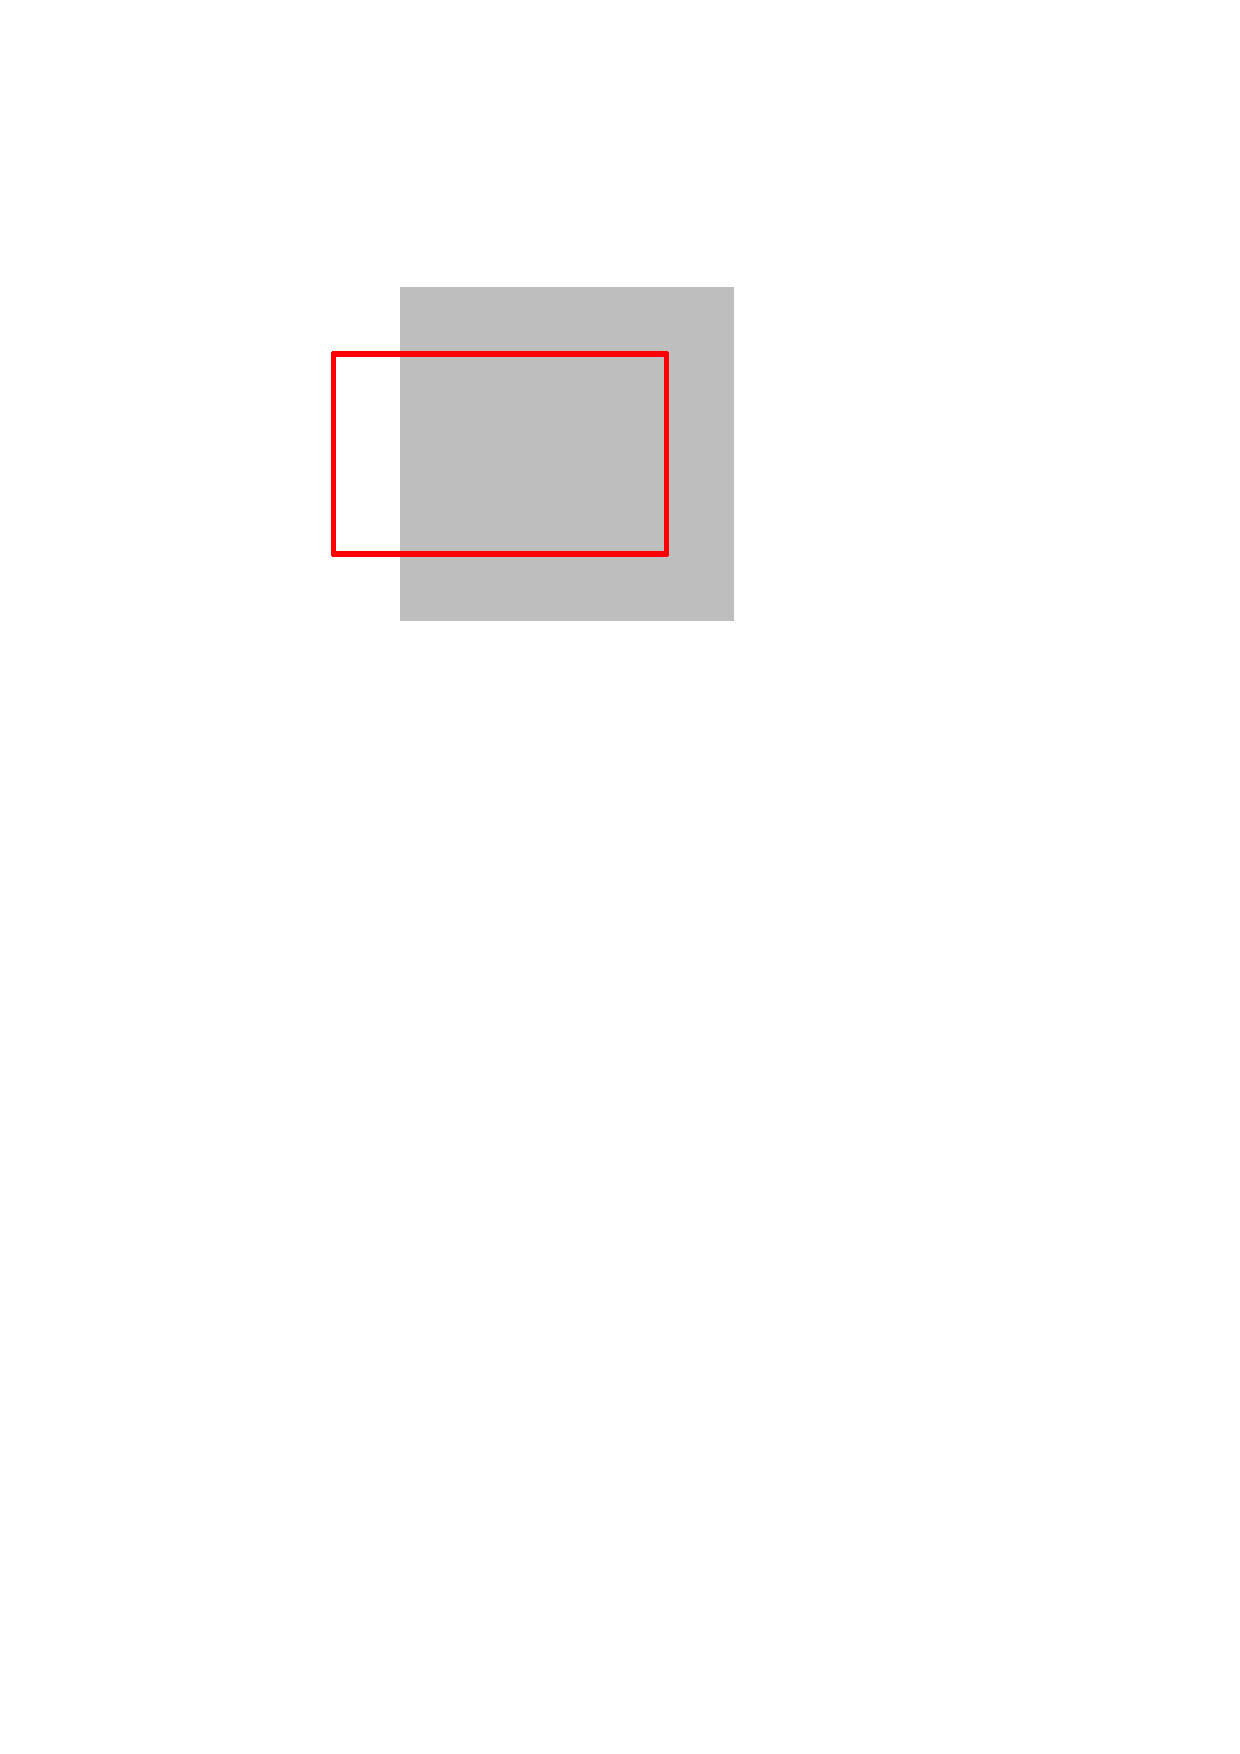
\includegraphics[scale=0.5,page=1]{fig/filter}
	\hfil
	\includegraphics[scale=0.5,page=2]{fig/filter}
	\caption{Initially we can create a large number of \addEs because of the segment tree structured, but after filtering the overhead is reduced.}\label{fig:filter}
\end{figure}

Filtering can be done in linear time with respect to the number of unfiltered rectangles.
To see why, notice that there are only $O(n^2)$ possible coordinates that a corner of a rectangle can have.
We can group the rectangles by their corners into an array of size $O(n^2)$ and use the array to find matching pairs of rectangles to remove or merge.

To make the minimum link path computation efficient, we want to avoid reilluminating the same cells multiple times.
For the 2D minimum link paths this was done by turning cells into obstacles once enough steps have passed since the cell was first discovered.
This approach works also for 3D, but since there are $O(n^2)$ cells and clearing a rectangle from the unified tree requires $O(n\log n)$ steps, having to do the clear operations for all the cells would increase the time complexity significantly.

To overcome this problem, instead of limiting the reachable cells we limit the creation of \addEs.
We create \addEs for the next step when a plane sweep hits an obstacle.
If the illumination first reaches an obstacle face $o$ on step $k$, then after step $k+2$ all the points touching $o$ are illuminated, so after step $k+3$ all the points visible from $o$ are illuminated.
Thus we don't create any \addEs for an obstacle $o$ that was first found more than 3 steps ago, as any point illuminated through such events has been illuminated already.

\subsection{Complexity}

We now prove the complexity of the minimum link computation algorithm.

\begin{lem}\label{lem:obse3}For each obstacle we generate \obsE on at most 9 steps of the illumination.\end{lem}
\begin{proof}
Recall that we stop generating \addEs from obstacles after 3 steps have passed since that obstacle was discovered.
Suppose we first generate \obsE for obstacle $o$ on step $k$.
After step $k+3$ all the points visible from $o$ are illuminated.
After step $k+4$ we have discovered each obstacle $h$ such that the illumination reaching $h$ could generate an \addE that illuminates $o$.
We won't generate any \addEs for such obstacle $h$ after step $k+7$, so the last time a sweep can reach $o$ is on step $k+8$.
\end{proof}

\begin{lem}\label{lem:celle3}For each cell we generate \cellE on at most 9 steps of the illumination.\end{lem}
\begin{proof}
The proof is very similar to Lemma~\ref{lem:obse3}.
If we discover a cell $c$ on step $k$ then all the points visible from $c$ are illuminated after step $k+3$, so no more sweeps can reach $c$ after step $k+8$.
\end{proof}

\begin{lem}\label{lem:adde3}The number of \addEs generated during the illumination after after filtering is $O(n^2)$.\end{lem}
\begin{proof}
We only count the \addEs in direction $+z$.
The other directions are identical.
Each \addE lies on the same plane with some obstacle face whose normal points to direction $-z$.
For the purpose of deriving an upper bound, we assume that each obstacle face has unique $z$-coordinate.
We may overcount the number of \addEs this way by counting the same events multiple times, but not undercount.

Consider the events on the plane $P$ of obstacle $o$ at $z$-coordinate $\hat{z}$.
Events in direction $+z$ can be generated during the sweeps to direction $\pm x$ and $\pm y$.
We only consider the sweep in direction $+y$.
We generate an event on plane $P$ if an \obsE removes a rectangle $R$ from the unified tree such that the upper $z$-coordinate of $R$ is $\hat{z}$.

Some \addEs might be generated on $P$ because of how the rectangles are stored in the unified segment tree.
When we add a rectangle to the tree it is split to canonical nodes, and some of them might have boundary on $P$.
In such cases we generate \addEs both from canonical nodes on both sides of $P$, so the events are removed during the filtering, where we remove pairs of events at identical positions that have opposite directions.

Because of the canonical nodes aligned with sides on $P$, we may also generate \addEs in direction $\pm x$ whose $z$-range is bounded by $\hat{z}$.
In the second part of the filtering we merge aligned events into larger events.
Because we generate the events on both sides of $P$, we will merge them so that the $z$-range of the combined event contains $\hat{z}$ but does not have endpoint on it.

Because of the filtering, we can only have events on plane $P$ after the sweep has reached obstacle $o$.
There are three cases for how an event might be generated on plane $P$ that is not removed by the filtering.
\begin{enumerate}
\item During a sweep in direction $+z$ we hit the obstacle $o$.
	We generate \addEs in directions $\pm x$ and $\pm y$ that are bounded by $\hat{z}$.
	From these \addEs we create events on plane $P$ on the following illumination step.
\item During a sweep in direction $\pm x$ or $\pm y$ the obstacle face $o$ cuts a rectangle in the tree such that the remaining part has boundary on $P$.
\item If on the previous step we created $\addE$ on plane $P$, then we also created events in directions $\pm x$ or $\pm y$ that have plane $P$ as one of the sides.
	From those events we create more $+z$ events on plane $P$ on the following step.
\end{enumerate}

First let us consider the first two types of events.
They only occur through sweeps touching the surface of obstacle $o$.
By Lemma~\ref{lem:obse3} and Lemma~\ref{lem:celle3} such sweeps occur only on $O(1)$ steps.
On a single sweep, the number of events created on $P$ is bounded by the number of canonical rectangles whose $z$-range is bounded by $\hat{z}$.
There are $O(n)$ such rectangles, so the number of events is $O(n)$.

Now consider the third type of events.
A crucial observation is the following:
After the illumination has reached obstacle $o$, the illumination on $P$ proceeds exactly like the 2D staged illumination in the cross section of $P$.
The 2D illumination illuminates maximal rectangles of \decomp{x} and \decomp{y}, producing a total of $O(n)$ illuminated rectangles.
There is some overhead because of reilluminating the same parts multiple times, but by Lemma~\ref{lem:celle3} each part of the domain can be illuminated only $O(1)$ times.

The number of events on the plane of a single obstacle $o$ is $O(n)$, so the total number of events is $O(n^2)$.
\end{proof}

We are ready to prove the main result of this section.

\begin{theo}Algorithm~\ref{alg:minlink3d} computes 3D minimum link path in $O(n^2\log^2n)$ time and $O(n^2)$ space.\end{theo}
\begin{proof}
By Lemma~\ref{lem:celle3} each cell is visited $O(1)$ times during the illumination.
On each \cellE we perform a single lookup to the unified tree in $O(\log^2 n)$ time, and iterate over the neighbors of the cell.
Since the decomposition has $O(n^2)$ cells and $O(n^2)$ links between cells, the total time taken in processing \cellEs is $O(n^2\log^2 n)$.

On each \addE we insert a new rectangle to the unified tree in $O(\log^2 n)$ time.
The filtering of \addEs can be done in linear time, and the total number of unfiltered events is at most the number of \addEs multiplied by the $O(\log^2 n)$ canonical nodes used to store a rectangle in the unified tree.
Thus the time complexity of the filtering is $O(n^2\log^2 n)$.

On each \obsE we clear a rectangle from the tree.
The clearing takes $O(n\log n + k)$ time, where $k$ is the number of cleared canonical rectangles.
Each \addE adds $O(\log^2 n)$ canonical rectangles to the tree, so the total number of rectangles to be cleared is $O(n^2\log^2 n)$.
There are $O(n)$ \obsEs by Lemma~\ref{lem:obse3}, so the total time taken in \obsEs is $O(n^2\log^2 n)$.

As all parts of the algorithm are done in $O(n^2\log^2 n)$ time, the total time complexity is $O(n^2\log^2 n)$.

The size of the decomposition as well as the segment tree used during the sweeps is $O(n^2)$, so the space complexity is $O(n^2)$.
\end{proof}

\subsection{Higher dimensional paths}

The algorithm for 3D minimum link paths can be generalized to higher dimensions.
We now assume that \fspace is a $D$-dimensional rectilinear region for arbitrary fixed $D\ge 2$.
We develop a generalization of Algorithm~\ref{alg:minlink3d} that computes the rectilinear minimum link path in $D$-dimensional space in $O(n^{D-1}\log^{D-1}n)$ time.

The algorithm uses the same set of events during the sweeps in the $D$-dimensional space as were used in 3D space.
The 2D sweep plane is replaced by a $(D-1)$-dimensional hyperplane, so each event $e$ defines a $(D-1)$-dimensional hyperrectangle \hrectof{e} instead of \rectof{e}.

We use $D$-dimensional Unified segment tree to store the sweep hyperplane state during the sweeps.
The unified tree and the $D$-dimensional space decomposition allow us to use almost identical algorithm for the higher dimension case as the algorithm for the 3D domains.

\begin{alg}\label{alg:sweepdd}
Illuminate by plane sweep in direction $+D$ starting from a provided event set $E$.
\begin{algorithmic}
\State $Q\gets$ Priority queue containing $E$.
\State $T\gets$ Empty $(D-1)$-dimensional Unified segment tree.
\While{$Q$ is not empty}
	\State $e\gets\pop{Q}$.
	\If{$e$ is \addE}
		\State Insert \hrectof{e} to $T$.
	\ElsIf{$e$ is \cellE}
		\If{\hrectof{e} touches any hyperrectangle in $T$}
			\State $c\gets\cellof{e}$.
			\ForAll{$o\in\obsd{c}{D+}$}
				\State Insert \obsE for $o$ to $Q$.
			\EndFor
			\ForAll{$b\in\nbsd{c}{D+}$}
				\State Insert \cellE for $b$ to $Q$.
			\EndFor
		\EndIf
	\ElsIf{$e$ is \obsE}
		\State Clear \hrectof{e} from $T$.
		\State Generate \addEs for the cleared canonical hyperrectangles.
	\EndIf
\EndWhile
\end{algorithmic}
\end{alg}

Using the hyperplane sweep, the $D$-dimensional minimum link path computation works as the following.

\begin{alg}\label{alg:minlinkdd}
Run staged illumination in $D$-dimensional domain \fspace starting from point \spt.
\begin{algorithmic}
\State Compute decomposition of \fspace into $D$-dimensional cells using Algorithm~\ref{alg:splitdd}.
\ForAll{$d\in\set{\pm1,\dots,\pm D}$}
	\State $E_d\gets$ Event set containing \addE at \spt and \cellE for the cell containing \spt.
\EndFor
\While{$E_d$ is not empty for some $d$}
	\ForAll{$d\in\set{\pm1,\dots,\pm D}$}
		\State $E_d'\gets$ Empty event set.
	\EndFor
	\ForAll{$d\in\set{\pm1,\dots,\pm D}$}
		\State Illuminate in direction $d$ using Algorithm~\ref{alg:sweep3d} with events $E_d$.
		\State Store the events generated by the sweep into $E_e'$ for $e\neq\pm d$.
	\EndFor
	\ForAll{$d\in\set{\pm1,\dots,\pm D}$}
		\State $E_d\gets E_d'$.
	\EndFor
\EndWhile
\end{algorithmic}
\end{alg}

We use the same method for avoiding reilluminating the same areas many times as was used in the 3D algorithm.
For each obstacle $o$ we record when it was first discovered, and use that to stop generating \addEs from $o$ after a certain number of steps has passed.
If $o$ is reached first on step $k$, then at the end of step $k+D$ all the points visible from $o$ are illuminated, so we can stop creating \addEs from $o$ starting from step $k+D+1$.

We also need to perform the filtering described in Section~\ref{sec:evtgen} to avoid generating a large number of \addEs because of the unified tree structure.
The filtering rules are exactly the same as the ones used in the 3D algorithm, except that we are working with $(D-1)$-dimensional hyperplanes.
The operations below are performed to \addEs produced by sweep in direction $+D$.
\begin{enumerate}
\item Remove all the pairs of \addEs with the same position but opposite direction.
\item Merge all sets of aligned \addEs with the same $D$-range into a single larger \addE.
\end{enumerate}

The definition of aligned \addEs is a bit more complicated in high-dimensional case.
A pair of \addEs can be aligned along multiple axes.
For two \addEs to be aligned, they need to in the event set for the same direction, and share the same coordinate where the events occur.
Let $a$ be any axis other than $D$.
The events are aligned in direction $a$ if the bounds of their hyperrectangles are identical in all the directions except $a$, and the bounds in direction $a$ touch each other at endpoints.

The filtering step allows us to again bound the number of \addEs processed during the illumination.

\begin{lem}\label{lem:obsed}For each obstacle we generate \obsE on at most $2D+3$ steps of the illumination.\end{lem}
\begin{proof}
The proof is similar to Lemma~\ref{lem:obse3} for the 3D case.
We stop generating \addEs from obstacles after $D$ steps have passed since that obstacle was discovered.
Suppose we first generate \obsE for obstacle $o$ on step $k$.
After step $k+D$ all the points visible from $o$ are illuminated.
After step $k+D+1$ we have discovered each obstacle $h$ such that the illumination reaching $h$ could generate an \addE that illuminates $o$.
We won't generate any \addEs for such obstacle $h$ after step $k+2D+1$, so the last time a sweep can reach $o$ is on step $k+2D+2$.
\end{proof}

\begin{lem}\label{lem:celled}For each cell we generate \cellE on at most $2D+3$ steps of the illumination.\end{lem}
\begin{proof}
The proof is very similar to Lemma~\ref{lem:obsed}.
If we discover a cell $c$ on step $k$ then all the points visible from $c$ are illuminated after step $k+D$, so no more sweeps can reach $c$ after step $k+2D+2$.
\end{proof}

\begin{lem}\label{lem:added}The number of \addEs generated during the illumination after after filtering is $O(n^{D-1})$.\end{lem}
\begin{proof}
The proof is similar to Lemma~\ref{lem:adde3}.
We only count the \addEs in direction $+D$ occurring on a hyperplane $P$ defined by a $(D-1)$-dimensional obstacle face $o$ that has $D$-coordinate $\hat{d}$.
To simplify the counting we assume that the obstacle $D$-coordinates are unique so $o$ is the only obstacle face on $P$.

We classify the events remaining after filtering similarly to the 3D case:
\begin{enumerate}
\item During a sweep in direction $+D$ we hit the obstacle $o$.
	We generate \addEs in directions other than $\pm D$ that are bounded by $\hat{d}$.
	From these \addEs we create events on plane $P$ on the following illumination step.
\item During a sweep in direction other than $\pm D$ the obstacle face $o$ cuts a hyperrectangle in the tree such that the remaining part has boundary on $P$.
\item If on the previous step we created $\addE$ on plane $P$, then we also created events in directions other than $\pm D$ that have plane $P$ as one of the sides.
	From those events we create more $+D$ events on plane $P$ on the following step.
\end{enumerate}

Similar to the 3D case, a single sweep can only produce as many events on $P$ as the number of canonical hyperrectangles bounded by $P$, which in the $(D-1)$-dimensional unified tree is $O(n^{D-2})$.
By Lemma~\ref{lem:obsed} and Lemma~\ref{lem:celled} the illumination can only touch $o$ on $O(1)$ steps, so the number of type 1 and 2 events on $P$ is $O(n^{D-2})$.

We use induction on $D$ to prove the number of type 3 events.
The base case $D=2$ is proven by Lemma~\ref{lem:adde3}.

For $D\ge 3$ notice that again the illumination on the boundary of $P$ advances exactly like the $(D-1)$-dimensional illumination in the cross section of $P$.
By induction the $(D-1)$-dimensional illumination creates $O(n^{D-2})$ events.
Multiplying this by the number of times any cell can be visited gives an upper bound for the $D$-dimensional illumination on $P$.
Since there is only a constant factor overhead compared to the $(D-1)$-dimensional illumination, the number of type~3 events is $O(n^{D-2})$.

The number of events on the hyperplane of each obstacle is $O(n^{D-2})$, so the total number of events is $O(n^{D-1})$.
\end{proof}

We are now ready to state the final result.

\begin{theo}Algorithm~\ref{alg:minlinkdd} computes $D$-dimensional minimum link path in $O(n^{D-1}\log^{D-1}n)$ time and $O(n^{D-1})$ space.\end{theo}
\begin{proof}
By Lemma~\ref{lem:celled} each cell is visited $O(1)$ times during the illumination.
On each \cellE we perform a single lookup to the unified tree in $O(\log^{D-1} n)$ time, and iterate over the neighbors of the cell.
Since the decomposition has $O(n^{D-1})$ cells and $O(n^{D-1})$ links between cells, the total time taken in processing \cellEs is $O(n^{D-1}\log^{D-1} n)$.

On each \addE we insert a new rectangle to the unified tree in $O(\log^{D-1} n)$ time.
The filtering of \addEs can be done in linear time, and the total number of unfiltered events is at most the number of \addEs multiplied by the $O(\log^{D-1} n)$ canonical nodes used to store a hyperrectangle in the unified tree.

On each \obsE we clear a hyperrectangle from the tree.
By Lemma~\ref{lem:segurmtime} each clear operation takes $O(n^{D-2}\log n + k)$ time, where $k$ is the number of cleared canonical nodes.
Each \addE adds $O(\log^{D-1} n)$ canonical rectangles to the tree, so the total number of rectangles to be cleared is $O(n^{D-1}\log^{D-1} n)$.
There are $O(n)$ \obsEs by Lemma~\ref{lem:obsed}, so the total time taken in \obsEs is $O(n^{D-1}\log^{D-1} n)$.

All parts of the algorithm are done in $O(n^{D-1}\log^{D-1} n)$ time, so the total time complexity is $O(n^{D-1}\log^{D-1} n)$.

The decomposition and the unified segment tree both require $O(n^{D-1})$ memory, so the space complexity is $O(n^{D-1})$.
\end{proof}



\section{Conclusions}\label{sec:conclusions}

We have discussed algorithms for the rectilinear minimum link path problem in two, three and higher dimensions.
We presented new algorithms for the problem with lower asymptotical running times than the previous known solutions.
The results are exciting since computing rectilinear minimum link paths is an old and well studied problem~\cite{wagner,restricted}.

We gave a simple algorithm for the planar rectilinear minimum link path problem with running time $O(n\log n)$~\cite{revisited}.
The algorithm has the same asymptotic complexity as older results~\cite{dasnar,sato}, but it uses simpler data structures.
We provided a new algorithm for the 3-dimensional variant of the problem with running time $O(n^2\log^2 n)~\cite{restricted}$.
We also showed that this result can be generalized to work for any dimension $D$ with running time $O(n^{D-1}\log^{D-1}n)$.
The new algorithms provide significant improvements over the previous best known results $O(n^{2.5}\log n)$~\cite{wagner} and $O(n^D\log n)$~\cite{de1992}.

The key techniques for achieving the new results were the recursive space decomposition (Sec.~\ref{sec:decomposition}) and the multidimensional segment tree (Sec.~\ref{sec:segtree}).
The algorithms are relatively simple, which is demonstrated by the implementation linked in Appendix~1.

A natural follow up question is whether the result could be improved further.
The planar problem was shown to be as difficult as sorting the input~\cite{dasnar}, so the known result are asymptotically optimal.
For the higher dimensional versions no other lower bound is known besides the $O(n\log n)$ bound.
The planar minimum link path problem without orientation restriction was shown to be 3SUM hard-hard by Mitchell, Polishchuk and Sysikaski~\cite{revisited}, but there is no known way to extend the result to the rectilinear case.

The bottleneck of the algorithm for $D$-dimensional minimum link path computation are the operations on the unified segment tree.
Thus the running time of the algorithm could be improved by developing a faster data structure for hyperrectangle intersection testing.
Wagner~\cite{unified} suggest that it might be possible to speed up the operations on the unified tree by a logarithmic factor through the use of fractional cascading.
However the idea is not discussed in detail, so developing a faster multidimensional segment tree varient remains as a future challenge.



\nocite{*}
\bibliographystyle{tktl}
\bibliography{ref}

\lastpage

\appendices

\pagestyle{empty}

\internalappendix{1}{Source code location}\label{apx:src}

An implementation of the high-dimensional rectilinear minimum link path algorithm presented in the thesis is available in the following URL: \\
\url{https://github.com/sisu/gradu/tree/master/code}

The code implements the minimum link path computation in time $O(n^{D-1}\log^{D-1}n)$ for a any constant $D$ defined at compile time.
The code is written in standard C++ using the C++14 standard.
The implementation does not depend on any libraries besides the C++ standard library, but the associated unit tests are written using the Google Test framework.

\end{document}


